\documentclass[a4paper]{report}
\usepackage{amsmath}

\usepackage{algpseudocode}
\usepackage[utf8]{inputenc}
\usepackage{vntex}
\usepackage[english]{babel}
\usepackage[table]{xcolor}
% \usepackage{enumitem}
\usepackage{amsfonts}
\usepackage{amssymb}
\usepackage{graphicx}
\usepackage[hang,flushmargin]{footmisc} % For hanging footnotes
\usepackage{setspace} % For fine spacing adjustments
\usepackage[font=normalsize]{caption}
\usepackage{booktabs}
\usepackage[unicode]{hyperref}
\usepackage[left=3cm,right=2cm,top=2.5cm,bottom=3cm]{geometry}
\usepackage{titlesec}
\usepackage{mdframed}
\usepackage{lipsum} % For example text (if needed)
\usepackage{colortbl}
\usepackage{booktabs}
\usepackage{array}
\usepackage{xcolor}
\usepackage{scrextend}
\usepackage{enumerate}
\usepackage{tikz}
\usepackage{float}
\usepackage{afterpage}
\usepackage{multirow}
\usepackage{multicol}
\usepackage{sectsty}
\usepackage{tocloft,calc}
\usepackage{listings}
\usepackage{makecell}
\usepackage{tocloft}
\usepackage{tcolorbox}
\usepackage{mathptmx}
\usepackage{longtable} % Include this in the preamble
\usepackage{inconsolata}  % Font monospace đẹp cho code
\usepackage{csquotes}
\usepackage{lmodern}
\usepackage{tabularx} % Add to preamble if not already there

% Định nghĩa màu
\definecolor{orange}{RGB}{255,128,0}
\definecolor{gray}{RGB}{128,128,128}
\definecolor{purple}{RGB}{128,0,128}

\usetikzlibrary{calc}
\usepackage{algorithm}
\usepackage{perpage} %the perpage package
\MakePerPage{footnote} %the perpage package command
\PassOptionsToPackage{table}{xcolor}

\def\changemargin#1#2{\list{}{\rightmargin#2\leftmargin#1}\item[]}
\let\endchangemargin=\endlist

\changefontsizes{13pt}
% \bibliographystyle{unsrt}

\lstset{
  basicstyle=\ttfamily\scriptsize, % Match font size and style in the image
  breaklines=true, % Allow line breaks
  numbers=left, % Add line numbers to the left
  % numberstyle=\tiny, % Smaller font for line numbers
  frame=lines, % Add a frame around the code
  xleftmargin=20pt, % Adjust left margin for alignment
  tabsize=4, % Tab size for indentation
  showstringspaces=false, % Hide visible spaces in strings
  language=Prolog % Set the language to Prolog
}

%%% Code block style
\definecolor{codebackground}{rgb}{0.95,0.95,0.97}
\definecolor{codekeyword}{rgb}{0.13,0.29,0.53}
\definecolor{codecomment}{rgb}{0.25,0.5,0.35}
\definecolor{codestring}{rgb}{0.63,0.13,0.09}
\lstdefinestyle{toclstyle}{
  backgroundcolor=\color{codebackground},
  basicstyle=\ttfamily\scriptsize,
  breakatwhitespace=false,
  breaklines=true,
  captionpos=b,
  commentstyle=\color{codecomment},
  keywordstyle=\color{codekeyword}\bfseries,
  stringstyle=\color{codestring},
  numbers=left,
  numbersep=8pt,
  numberstyle=\tiny\color{gray},
  frame=single,
  rulecolor=\color{gray!30},
  showspaces=false,
  showstringspaces=false,
  showtabs=false,
  tabsize=2,
  morekeywords={context, inv, always, next, sometime, until, before, previous, 
                alwaysPast, sometimePast, since, implies, and, or, not, self, 
                isCalled, becomesTrue},
}

% Java code listing style - Add to preamble
% Java code listing style - Update string color
\definecolor{javakeyword}{rgb}{0.0, 0.0, 0.75}     % Dark blue for keywords
\definecolor{javacomment}{rgb}{0.5, 0.5, 0.5}      % Gray for comments
\definecolor{javastring}{rgb}{0.0, 0.6, 0.0}       % Changed to green for strings
\definecolor{javaannotation}{rgb}{0.6, 0.0, 0.6}   % Purple for annotations
\definecolor{javadoc}{rgb}{0.25, 0.5, 0.35}        % Forest green for javadoc
\definecolor{javabackground}{rgb}{0.98, 0.98, 1.0} % Very light blue background
\lstdefinestyle{javastyle}{
  language=Java,
  backgroundcolor=\color{white},
  basicstyle=\ttfamily\footnotesize,
  keywordstyle=\color{javakeyword}\bfseries,
  commentstyle=\color{javacomment}\itshape,
  stringstyle=\color{javastring},
  numberstyle=\tiny\color{gray},
  breakatwhitespace=false,
  breaklines=true,
  captionpos=b,
  keepspaces=true,
  numbers=left,
  numbersep=5pt,
  frame=none,
  rulecolor=\color{black},
  showspaces=false,
  showstringspaces=false,
  showtabs=false,
  tabsize=4,
  % Java-specific keywords
  morekeywords={String, TokenStream},
  % Handle annotations
  moredelim=[s][\color{javaannotation}]{@}{(},
  % Handle Javadoc comments
  morecomment=[s][\color{javadoc}]{/*}{*/},
  morecomment=[l][\color{javacomment}]{//},
}

\makeatletter
\def\l@figure{\@dottedtocline{1}{1em}{2.2em}}
\def\l@table{\@dottedtocline{1}{1em}{2.2em}}
\renewcommand*{\ALG@name}{Algorithm}
\makeatother

\sectionfont{\fontsize{15}{15}\selectfont}
\subsectionfont{\fontsize{13}{15}\selectfont}
\titleformat{\subsubsection}[runin]
{\normalfont\normalsize\bfseries}{\thesubsubsection.}{1em}{}
\titlespacing*{\subsubsection}{0pt}{*0.5}{*0.5}

% Include subsubsections in numbering and TOC
\setcounter{secnumdepth}{3}
\setcounter{tocdepth}{3}

\titleformat{\chapter}[display]
{\normalfont\huge\bfseries}{\chaptertitlename\ \thechapter}{0pt}{\LARGE}
\titlespacing*{\chapter}{0cm}{-\topskip}{20pt}[0pt]

\renewcommand{\baselinestretch}{1.3}
%\renewcommand{\cftsecpresnum}{Chương\space}
\renewcommand{\cftchappresnum}{Chapter }
\AtBeginDocument{\addtolength\cftchapnumwidth{\widthof{\bfseries Chapter}}}
\setlength{\parskip}{0.4em}
\setlength{\parindent}{0pt}


% Tùy chỉnh định dạng mục lục
\renewcommand{\cftchappresnum}{Chapter }
\renewcommand{\cftchapaftersnum}{: }

\setlength{\cftchapnumwidth}{2.5em}

%
\newcommand{\argmax}{\arg\!\max}
\usepackage[
  backend=biber,
  sorting=ynt
]{biblatex}
\addbibresource{references.bib}


\usepackage{graphicx}
\usepackage{array}
\graphicspath{ {figures/} }

\renewcommand{\listfigurename}{List of plots}
\renewcommand{\listtablename}{Tables}

%%%%%%%%%%%%%%%%%%%%%%%%%%%%%%%%%%%%%%%%%%%%%%%%%%%%%%%%%%%%%%%%%%%%%%%%%%%%%%%%%%%%%%%%%%%%%%%%%%%%%%%
\begin{document}
\newcommand\setfontsize[1]{\fontsize{#1}{1.3\dimexpr#1}\selectfont}

% Cover english
\pagenumbering{gobble}

\begin{center}
	\begin{tikzpicture}[overlay,remember picture]
		\draw[line width=3pt,color=black,fill=none]
		($(current page.north west)+(2.5cm,-2cm)$) rectangle
		($(current page.south east)-(1.5cm,-2.5cm)$);
		\draw[line width=1pt,color=black,fill=none]
		($(current page.north west)+(2.65cm,-2.15cm)$)
		rectangle ($(current page.south east)-(1.65cm,-2.65cm)$);
	\end{tikzpicture}
	\\[1mm]
	\setfontsize{12pt}\textbf{VIETNAM NATIONAL UNIVERSITY, HANOI
		\\UNIVERSITY OF ENGINEERING AND TECHNOLOGY}\\[2cm]
	
\includegraphics[width=0.2\linewidth]{figures/uet.jpg}\\[0.5cm]
	\setfontsize{14pt}\textbf{}
	\\[1.5cm]
	\setfontsize{18pt}\textbf{PHÁT TRIỂN HỆ THỐNG TẠO LẬP VÀ QUẢN LÝ GIAO
		DỊCH ĐỒNG TIỀN ĐIỆN TỬ PHI TẬP TRUNG  \\TRÊN NỀN TẢNG ĐA CHUỖI KHỐI}
	\\[2cm]
	\setfontsize{14pt}\textbf{KHÓA LUẬN TỐT NGHIỆP
		\\
		Chuyên ngành: Khoa học máy tính }

	\vfill
	\setfontsize{12pt}\textbf{HÀ NỘI – 2025}
\end{center}

\newpage

% \begin{center}
\begin{tikzpicture}[overlay,remember picture]
	\draw[line width=3pt,color=black,fill=none]
	($(current page.north west)+(2.5cm,-2cm)$) rectangle
	($(current page.south east)-(1.5cm,-2.5cm)$);
	\draw[line width=1pt,color=black,fill=none]
	($(current page.north west)+(2.65cm,-2.15cm)$)
	rectangle ($(current page.south east)-(1.65cm,-2.65cm)$);
\end{tikzpicture}
\\[1mm]
{
\centering
\setfontsize{12pt}\textbf{VIETNAM NATIONAL UNIVERSITY, HANOI
	\\UNIVERSITY OF ENGINEERING AND TECHNOLOGY}\\[1.5cm]
\setfontsize{14pt}\textbf{Trần Chiến Thắng}
\\[1.5cm]
\setfontsize{18pt}\textbf{PHÁT TRIỂN HỆ THỐNG TẠO LẬP VÀ QUẢN LÝ GIAO
	DỊCH ĐỒNG TIỀN ĐIỆN TỬ PHI TẬP TRUNG  \\TRÊN NỀN TẢNG ĐA CHUỖI KHỐI}
\\[3cm]
\setfontsize{14pt}\textbf{KHÓA LUẬN TỐT NGHIỆP \\
	Chuyên ngành: Khoa học máy tính}\\[3cm]
}

\hspace*{8mm}\setfontsize{14pt}\textbf{Giảng viên hướng dẫn: PSG.TS.
	Đặng Đức Hạnh}\\[0.8cm]

\begin{center}
	\vfill
	\setfontsize{12pt}\textbf{HÀ NỘI – 2025}
\end{center}
% \end{center}

% \begin{center}

% 	\begin{tikzpicture}[overlay,remember picture]
% 		\draw[line width=3pt,color=black,fill=none]
% 			($(current page.north west)+(2.5cm,-2cm)$) rectangle ($(current page.south east)-(1.5cm,-2.5cm)$);
% 		\draw[line width=1pt,color=black,fill=none]
% 			($(current page.north west)+(2.65cm,-2.15cm)$) rectangle ($(current page.south east)-(1.65cm,-2.65cm)$);
% 	\end{tikzpicture}
% 	\\[1mm]
% 	\textbf{VIETNAM NATIONAL UNIVERSITY, HANOI \\UNIVERSITY OF ENGINEERING AND TECHNOLOGY}
% 	\\[1cm]
% 	\\[0.3cm]
% 	\textbf{Dang Tran Hoang Ha}
% 	\\[2cm]

% 	\large{\textbf{A SAT APPROACH FOR SOLVING \\SOCIAL GOLFER PROBLEM - SGP}}
% 	\\[2.6cm]
% 	\normalsize{\textbf{BACHELOR’S THESIS
% 		\\[2mm]
% 	Major: Information Technology}}
% \end{center}
% \vspace{16mm}
% \hspace*{12mm}\textbf{ Supervisor: PhD. To Van Khanh}\\[0.8cm]

% \vfill
% \begin{center}
% 	\textbf{HA NOI – 2024}
% 	\vspace{10mm}
% \end{center}\newpage\cleardoublepage

% Abstract Vietnamese
% \begin{center}
  \textbf{\large{TÓM TẮT}	}
\end{center}

\addcontentsline{toc}{chapter}{TÓM TẮT}

\begin{small}

  \textbf{Tóm tắt:} Khóa luận tập trung nghiên cứu và phát triển ứng dụng
  LaunchCrypt,
  một nền tảng đổi mới trong lĩnh vực tài chính phi tập trung (DeFi), nhằm đơn
  giản hóa
  quá trình tạo và giao dịch token cho người dùng không có kiến thức chuyên sâu
  về
  công nghệ. Để xây dựng nền tảng này, khóa luận đề xuất sử dụng stack công
  nghệ hiện
  đại bao gồm ReactJS cho phần frontend, NestJS cho backend, và các ngôn ngữ
  lập
  trình hợp đồng thông minh như Move, Solidity, và Rust để hỗ trợ đa chuỗi. Bài toán
  chính mà
  khóa luận giải quyết là tạo ra một hệ sinh thái toàn diện cho việc tạo, giao
  dịch, và
  phát triển token một cách an toàn và hiệu quả. Để có thể hiểu và áp dụng đúng
  các
  công nghệ cho bài toán này, khóa luận trước tiên đã nêu một số kiến thức nền
  tảng về
  công nghệ chuỗi khối, hợp đồng thông minh, các nguyên lý hoạt động của DeFi, cũng như các
  giao thức
  và chuẩn token trên các chuỗi khối khác nhau. Sau khi tìm hiểu tất cả các
  kiến thức
  nền tảng liên quan, khóa luận vận dụng phát triển ba mô đun chính của
  LaunchCrypt:
  (1) mô đun tạo token, cho phép người dùng dễ dàng tạo ra token của riêng họ
  trên các
  chuỗi được hỗ trợ, (2) mô đun giao dịch token, tự động tạo cặp giao dịch
  và cung
  cấp giao diện cho việc mua bán token, và (3) mô đun tốt nghiệp token, quản lý
  quá
  trình chuyển token lên các sàn giao dịch phi tập trung lớn hơn khi đạt đủ
  thanh khoản.
  Bên cạnh đó, khóa luận cũng phát triển các tính năng bổ sung như stake token,
  khả năng tương tác, kết nối giữa các đối tượng người dùng cùng với khả năng hỗ
  trợ đa chuỗi, bao gồm Aptos, Solana và Avalanche. Điều này không chỉ mở rộng
  phạm vi tiếp cận của dự án mà còn thúc đẩy tính linh hoạt và khả năng tương tác
  giữa các chuỗi khối khác nhau. Bằng
  cách cung cấp các công cụ như giao diện Tradingview cho giao dịch nâng cao,
  tính năng
  mua/bán tự động và thông tin chi tiết về token, LaunchCrypt không chỉ phục vụ
  người
  dùng mới mà còn đáp ứng nhu cầu của các nhà giao dịch có kinh nghiệm. Hơn
  nữa,
  việc tích hợp với các giải pháp để hỗ trợ người dùng Web 2.0 thể hiện tầm
  nhìn dài hạn
  của dự án trong việc thu hẹp khoảng cách giữa tài chính truyền thống và DeFi.
  Cuối
  cùng, khóa luận sẽ đề cập cách triển khai và thử nghiệm nền tảng LaunchCrypt
  trên
  môi trường thực tế, đánh giá hiệu quả của giải pháp trong việc giải quyết các
  thách
  thức của DeFi, và đưa ra các kết luận cũng như hướng phát triển tiếp theo cho
  dự án.

  \textbf{Từ khóa}: \textit{LaunchCrypt, DeFi, Aptos, Solana,
    Avalanche, ReactJS, NestJS, Move, Solidity, Rust, Tradingview, Web 2.0}

  % \vspace*{1cm}
  % \textbf{Keywords}: \textit{SGP, SAT, SAT Encoding, CNF Encoding.}

\end{small}\newpage\cleardoublepage
% Abstract English
\begin{center}
  \textbf{\large{ABSTRACT}	}
\end{center}

\addcontentsline{toc}{chapter}{ABSTRACT}

\begin{small}

\textbf{Abstract:} In Model-Driven Engineering (MDE), models serve as primary artifacts 
for abstracting and designing software systems. The Unified Modeling Language (UML) and 
the Object Constraint Language (OCL) are widely used for specifying structural and 
behavioral properties of these models. However, OCL has fundamental limitations in 
expressing properties that span multiple system states or involve event occurrences, 
making it challenging to specify and verify dynamic aspects of systems. This thesis 
addresses these limitations by introducing TOCL+ (Temporal OCL+), an extension of OCL 
with temporal operators and event constructs. TOCL+ enables developers to specify 
complex temporal properties such as safety and liveness constraints using familiar 
OCL syntax, while incorporating temporal logic concepts. We present a systematic 
transformation approach that converts TOCL+ expressions into standard OCL constraints 
interpreted over filmstrip models—representations of system execution paths as 
sequences of snapshots. This transformation enables verification of temporal 
properties using existing OCL tools without requiring specialized temporal logic
model checkers. We implement this approach as a plugin for the UML-based Specification 
Environment (USE) tool and demonstrate its effectiveness through a software system 
case study, showing how our approach bridges the gap between intuitive temporal 
specification and practical model verification.
  
\textbf{Keywords}: \textit{Model-Driven Engineering, Object Constraint Language, 
Temporal Properties, Event Specification, Model Verification, Filmstrip Models, 
OCL Extensions, USE Tool, Formal Verification}

\end{small}\newpage\cleardoublepage
% Assurance
\setlength{\parindent}{1cm}

\begin{center}
  \textbf{\large{LỜI CAM ĐOAN}	}
\end{center}
\addcontentsline{toc}{chapter}{LỜI CAM ĐOAN}

Em – Trần Chiến Thắng, sinh viên QH-2021-I/CQ-CA-CLC2 Trường Đại học
Công Nghệ xin cam đoan khóa luận tốt nghiệp \textbf{\textit{“hát triển hệ thống
    tạo lập và quản lý giao dịch đồng tiền điện tử phi tập trung trên nền tảng đa
    chuỗi khối”}} là công trình em tự thực hiện dưới sự đầu tư nghiên cứu nghiêm
túc của bản thân và sự hướng dẫn của PGS.TS. Đặng Đức Hạnh. Trong khóa luận này
em có sử dụng lại một số đoạn mã nguồn mở cùng mô hình được thầy Hạnh cung cấp
và giúp đỡ chỉnh sửa lại cho phù hợp với đề tài mà mình nghiên cứu, sẽ không có
phần nào được sao chép từ tài liệu bên ngoài mà không được dẫn nguồn. Em xin
chịu mọi trách nhiệm về lời cam đoan này.

% \begin{changemargin}{10.9cm}{1cm}
% Hanoi, May 10, 2024
% \end{changemargin}

% \begin{changemargin}{12cm}{2cm}
% Signature
% \\[2cm]
% \end{changemargin}

% \begin{changemargin}{10.9cm}{1.3cm}
% Dang Tran Hoang Ha
% \end{changemargin}

\vspace{1cm}
\begin{flushright}
  \begin{minipage}{8cm}
    \centering
    Hà Nội, ngày 31 tháng 05 năm 2025\\[0.2cm]
    Sinh viên\\[2.5cm]

    Trần Chiến Thắng
  \end{minipage}
\end{flushright}\newpage\cleardoublepage
% Acknowledgement
\setlength{\parindent}{1cm}
\setcounter{page}{1}
\pagenumbering{roman}

\begin{center}
  \textbf{\large{ACKNOWLEDGEMENTS}	}
\end{center}
\addcontentsline{toc}{chapter}{ACKNOWLEDGEMENTS}

% Version 2
I would like to express my deepest gratitude to my supervisor, Assoc. Prof. Dang Duc Hanh, 
for his invaluable guidance and unwavering support throughout the research and 
writing of this thesis. His expertise and dedication have been instrumental in shaping this work.

I am also grateful to the alumni and current members of 
the research group for their insightful discussions and 
constructive feedback, which greatly enriched my research.

Furthermore, I extend my thanks to the faculty members of the University 
of Engineering and Technology for their passionate teaching and for 
equipping me with the essential knowledge and skills that form 
the foundation of this thesis.

Lastly, I offer my gratitude to my family for their constant 
care, support, and encouragement. Their belief in me provided 
the motivation and stability I needed to pursue and complete this 
thesis.

Although I have endeavored to conduct this research to 
the highest standard, I recognize that limitations in my knowledge 
and experience may have led to unintentional shortcomings. 
I sincerely welcome comments and suggestions from professors and peers 
to enhance this work further.

To all who have supported me on this journey, I am profoundly grateful.

% Version 1
% Under the assignment of the Faculty of Information Technology, 
% University of Engineering and Technology - VNU, and with the approval and guidance 
% of my supervisor - Assoc. Prof. Dang Duc Hanh, I have completed the thesis entitled: 
% \textbf{\textit{"A support tool to specify and verify temporal properties in OCL"}}.

% To complete this thesis, I would like to express my sincere gratitude 
% to my supervisor - Assoc. Prof. Dang Duc Hanh for his dedicated guidance and support both in the 
% research lab and throughout the course of this thesis.

% I would also like to thank the alumni and fellow members of the research group who have
% for their support and valuable discussions throughout the research process.

% Then, I would like to express my gratitude to the faculty members of the University of
% Engineering and Technology for their dedicated and enthusiastic teaching, which has
% provided me with valuable foundational knowledge.

% Lastly, I would like to express my heartfelt gratitude to my family for their care, 
% support, and encouragement, which have provided me with the motivation 
% and favorable conditions to study and complete this thesis with peace of mind.

% Although I have made every effort to carry out this research to the best of my ability, 
% due to limitations in my knowledge and experience, 
% this thesis may still contain shortcomings that I may not have recognized. 
% I sincerely welcome any comments and suggestions from professors 
% and fellow students to help improve this work.

% I would like to extend my deepest thanks.
\newpage\cleardoublepage


\addcontentsline{toc}{chapter}{TABLE OF CONTENTS}
\renewcommand{\contentsname}{\centering \fontsize{22}{0}\selectfont \bfseries TABLE OF CONTENTS}
\tableofcontents\newpage\cleardoublepage
%

\newpage
\addcontentsline{toc}{chapter}{LIST OF FIGURES}
\renewcommand{\listfigurename}{\centering \fontsize{22}{0}\selectfont \bfseries LIST OF FIGURES}
\listoffigures\cleardoublepage

\newpage
\addcontentsline{toc}{chapter}{LIST OF TABLES}
\renewcommand{\listtablename}{\centering \fontsize{22}{0}\selectfont \bfseries LIST OF TABLES}
\listoftables

\newpage
\chapter*{ABBREVIATION AND TERMS}
\addcontentsline{toc}{chapter}{ABBREVIATION AND TERMS}

%\begin{tabular}{|l|l|l|l|}
\begin{longtable}{|>{\raggedright\arraybackslash}p{4cm}|>{\raggedright\arraybackslash}p{10cm}|}
  \hline
  \textbf{Abbreviation}       & \textbf{Full Form}           
  \\
  \hline
  MDE                    & Model Driven Engineering  
  \\
  \hline
  UML                    & Unified Modeling Language    
  \\
  \hline
  OCL                    & Object Constraint Language
  \\
  \hline
  USE                    & UML-based Specification Environment
  \\
  \hline
  TOCL                   & Temporal Object Constraint Language
  \\
  \hline
  TOCL+                  & Temporal Object Constraint Language Plus
  \\
  \hline
\end{longtable}\newpage\cleardoublepage
%\listoftables

%
\setcounter{page}{1}

\pagenumbering{arabic}

\setlength{\parindent}{1cm}

\begin{center}
  \section*{INTRODUCTION}
\end{center}
\addcontentsline{toc}{chapter}{INTRODUCTION}

% \subsection*{Background and Significance of the Study}

\hspace{\parindent}Model-Driven Engineering (MDE) approaches system development 
by emphasizing models over source code. Through modeling languages such as UML 
and OCL, developers construct models that abstract the system complexity and serve as primary development artifacts. 
These models can then be transformed into executable code, documentation, and test cases using automated 
model transformation techniques. Techniques like validation and verification help 
ensure the models’ quality, with structural aspects, represented by class and object 
diagrams, being particularly important.

The Unified Modeling Language (UML) offers a standard way to create diagrams that show 
a system’s structure and behavior, while the Object Constraint Language (OCL) adds precise 
rules to these models. OCL uses simple logic to define conditions that must always be true 
or requirements for operations. However, it lacks the expressive power to model temporal properties 
that involve different states of the model or depend on event occurrences. 
This limitation stems from the absence of built-in constructs for handling time and events in OCL.

% \subsection*{Research Objectives}

In this work, we aim to extend OCL to support temporal properties and events,

\hspace{\parindent}

% \subsection*{Research Methodology}
Để đạt được các mục tiêu trên, khóa luận sẽ áp dụng các phương pháp nghiên cứu
sau:
% \begin{itemize}
%   \item \textbf{Nghiên cứu lý thuyết}:

%   \item \textbf{Phát triển phần mềm}: 

%   \item \textbf{Thử nghiệm và đánh giá}:
% \end{itemize}

% \subsection*{Structure of the Thesis}
Cấu trúc khóa luận gồm 4 phần như sau:
\begin{itemize}
  \item \textbf{Chương 1}: 

  \item \textbf{Chương 2}: 

  \item \textbf{Chương 3}: 

  \item \textbf{Kết luận}: 
\end{itemize}

% Model-driven engineering (MDE) takes a view on system development focusing on
% models than on code. Using modeling languages like UML and OCL, developers create models 
% that abstract the system’s complexity and serve as the central artifacts 
% in MDE. From these models, code, documentation, and test cases can be 
% automatically generated through model transformations. Techniques like validation 
% and verification help ensure the models’ quality, with structural aspects - 
% represented by class and object diagrams - being particularly important.

% Traditional software engineering, reliant on manual coding, 
% struggles with increasingly large, complex projects despite aiming for reliable and efficient systems. 
% This causes inefficiencies not from software requirements but from development 
% process limitations, driving the need for simpler, more flexible approaches. 
% To address these challenges, 
% Model Driven Engineering (MDE) \cite{MDE} offers a promising methodology 
% aimed at reducing accidental complexities by focusing on models over code. 
% Using modeling languages like UML and OCL, developers create models 
% that abstract the system’s complexity and serve as the central artifacts 
% in MDE. From these models, code, documentation, and test cases can be 
% automatically generated through model transformations. Techniques like validation 
% and verification help ensure the models’ quality, with structural aspects - 
% represented by class and object diagrams - being particularly important.

% Software engineering aims to build reliable and 
% efficient systems, but as projects become larger and more complex, 
% traditional development methods face many challenges. These methods 
% often rely heavily on manual coding, which can’t always keep up with 
% growing demands. As a result, problems and inefficiencies can occur—not 
% because of the software’s requirements, but because of how the 
% development process is handled. This shows the need for new approaches 
% that can make development easier and more flexible.
\newpage\cleardoublepage
\chapter{Backgrounds}

\setlength{\parindent}{1cm}

\section{Introduction}

\hspace{1cm} This chapter presents fundamentals about concepts and artifacts essential 
to this thesis. The modeling languages such as, Unified Modeling Language (UML), 
together with Object Constraint Language (OCL), are used to describe structural and 
behavioral aspects of systems and are briefly described in this chapter. A description 
of the modeling and specification tool called UML-based Specification Environment (USE)
is presented, including its model validation capabilities that form the foundation for 
our verification approach. We explain the filmstrip model transformation process in 
detail, as it serves as the underlying mechanism for our temporal verification approach.

\section{Model-Driven Engineering}


\section{Unified Modeling Language (UML)}

\hspace{1cm} The Unified Modeling Language (UML) is a graphical language for 
visualizing, specifying, constructing, and documenting software-intensive systems.
This unified language is maintained by the Object Management Group (OMG) [58].

The UML has become one of the most widely used modeling language that can
be used with all significant object and component methods for describing real-world
application domains. Software systems, in today’s world, are growing in size, complex
ity, distribution and importance. As a result, building and maintenance of software
have become a more complex and challenging task. Therefore, the deployment of
languages such as UML reduces the complexity and difficulty by providing a high
level of abstraction, which describes precise and essential information for designing
and developing the software system [50].  

The graphical representation of the UML includes a set of diagrams, each focusing
on different aspects of a design. The UML Notation Guide states all the notation of 
diagram elements [58]. These diagrams can be classified into two groups (a) a structural
diagram that represents the static aspect of the system, and (b) a behavioral diagram
that describes the dynamic aspect of the system. Altogether, fourteen different model
types can be found in the Unified Modeling Language Reference Manual [71]. In this
thesis, three diagrams, i.e., class diagram, object diagram and sequence diagram, have
been extensively used and are explained further in this section.

\subsection{Class Diagram}

\subsection{Object Diagram}

\subsection{Sequence Diagram}
\section{Object Constraint Language (OCL)}
\label{sec:ocl}

\subsection{Overview}

\hspace{1cm} As explained in the previous section, UML is a graphical language for 
visualizing system structure and behavior. However, visual modeling with UML alone 
is insufficient for developing accurate and consistent software models, as UML 
diagrams cannot express all necessary constraints. The Object Management Group (OMG) 
developed the Object Constraint Language (OCL) to address this limitation \cite{OCL}. 
OCL is a formal assertion language with precise semantics that extends UML by 
allowing developers to specify constraints that cannot be expressed graphically. 

\begin{figure}
    \begin{center}
        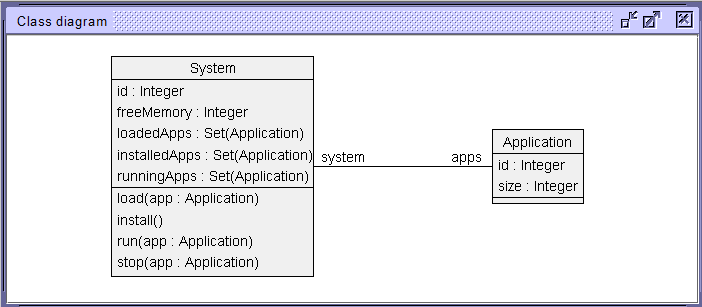
\includegraphics[width=0.8\textwidth]{figures/c1/SoftwareSystem/SS_Ver2_Gray.png}
        \caption{Class diagram of the Software System.}
        \label{fig:class_diagram_software_system}
    \end{center}
\end{figure}

To demonstrate OCL's capabilities, we'll use a simple software system model shown 
in Figure \ref{fig:class_diagram_software_system}. This model contains two classes: 
\texttt{System} and \texttt{Application}. Each class has an \texttt{id} attribute 
for unique identification. The \texttt{System} class has a \texttt{freeMemory} attribute 
representing available memory, while each \texttt{Application} has a \texttt{size} 
attribute indicating its memory requirements. The \texttt{System} class maintains three 
collections: \texttt{loadedApps}, \texttt{installedApps}, and \texttt{runningApps}, which 
track applications in different states throughout their lifecycle.

The \texttt{System} class defines the following operations:
\begin{itemize}
    \setlength{\itemsep}{0pt}
    \setlength{\parskip}{0pt}
    \setlength{\parsep}{0pt}
    \item \texttt{load(app : Application)}: downloads the application \textit{app} given as parameter and adds it to the \texttt{loadedApps} collection.
    \item \texttt{install()}: installs all the loaded applications in the \texttt{loadedApps} collection and moves them to the \texttt{installedApps} collection.
    \item \texttt{run(app : Application)}: executes the application \textit{app} given as a parameter that should be installed, adding it to the \texttt{runningApps} collection.
    \item \texttt{stop(app : Application)}: stops the application \textit{app} given as a parameter that should be running, removing it from the \texttt{runningApps} collection.
\end{itemize}


\subsection{OCL Constraints}
\hspace{1cm} Listing \ref{lst:ocl_constraints} demonstrates three typical aspects of OCL constraints. 
First, the \texttt{memoryConstraint} ensures system integrity by verifying that the 
system's free memory is non-negative, preventing memory overallocation. 
Second, the \texttt{notLoadedAndInstalled} constraint demonstrates OCL's ability to work with 
collections, ensuring that the sets of loaded and installed applications don't overlap - 
an application cannot be simultaneously in both states. This constraint uses the 
\texttt{intersection} and \texttt{isEmpty} operations to verify this condition.
Third, the \texttt{sizeConstraint} demonstrates how OCL can define 
simple rules that apply to all instances of a class, in this case ensuring all 
applications have a positive size.

\begin{lstlisting}[
    style=toclstyle, 
    caption={OCL constraints.}, 
    label={lst:ocl_constraints}
]
context System
inv memoryConstraint: self.freeMemory >= 0
inv notLoadedAndInstalled: self.loadedApps->intersection(self.installedApps)->isEmpty()

context Application
inv sizeConstraint: self.size > 0
\end{lstlisting}

OCL constraints typically appear in three forms:
\begin{itemize}
    \item \textbf{Invariants:} Conditions that must always be true for all instances 
    of a class throughout their lifetime, as shown in our examples above.
    
    \item \textbf{Preconditions:} Conditions that must be true before an operation 
    executes. For instance, we could specify that an application must not be in any
    collection before the \texttt{load} operation can be performed.
    
    \item \textbf{Postconditions:} Conditions that must be true after an operation 
    completes. For example, after executing the \texttt{load} operation, the application
    must be added to the \texttt{loadedApps} collection.
\end{itemize}

Listing \ref{lst:ocl_rules} demonstrates pre- and postconditions for the \texttt{load} 
operation. The preconditions verify that (1) the application is not already in any of the
three collections (\texttt{loadedApps}, \texttt{installedApps}, or \texttt{runningApps}) 
and (2) there is enough memory available for the application. The postconditions 
ensure that (1) the application is added to the \texttt{loadedApps} collection and (2) the 
available memory is reduced by the application's size.

\begin{lstlisting}[
    style=toclstyle, 
    caption={OCL rules.}, 
    label={lst:ocl_rules}
]
pre notLoaded: not self.loadedApps->includes(app) and
               not self.installedApps->includes(app) and
               not self.runningApps->includes(app)
pre enoughMemory: self.freeMemory >= app.size
post loaded: self.loadedApps = self.loadedApps@pre->including(app)
post freeMemory: self.freeMemory = self.freeMemory@pre - app.size
\end{lstlisting}

In the postcondition \texttt{freeMemory}, note the use of the \texttt{@pre} 
operator, which references the value of an attribute before the operation execution. 
This allows OCL to express constraints that relate the state before and after an 
operation. In this case, it ensures that the system's free memory after loading 
is reduced by exactly the size of the loaded application.

These examples represent just a small subset of OCL's expressive capabilities. 
OCL is type-rich, supporting basic types (Boolean, Real, Integer, String), collection 
types (Set, Bag, Sequence, OrderedSet), and special types (tuples, OclAny, OclType). 
The language provides powerful navigation capabilities for traversing relationships 
in the model, comprehensive collection operations for manipulating groups of objects, 
and quantifiers (forAll, exists) for building complex logical statements.

\subsection{OCL Limitations}

\subsubsection{Temporal Dimension}
\hspace{1cm} To illustrate the temporal limits of OCL, let us consider the following temporal 
properties of our software system: 

\begin{figure}
    \begin{mdframed}
        \item \textbf{Safety 1:} An application loading must precede its run.
        \item \textbf{Safety 2:} There must be an install operation between an application's loading and its running.
        \item \textbf{Safety 3:} Each application can be loaded at most one time.
        \item \textbf{Liveness:} Every loaded application will eventually be installed.
    \end{mdframed}        
    \captionof{figure}{Temporal properties of the software system.}
    \label{fig:temporal_properties}
\end{figure}

Such temporal properties are impossible to specify in OCL without at least enriching 
the model structure with state variables. In temporal logics, we formally distinguish 
safety properties (which prevent bad events/states) from liveness properties (which 
ensure good events/states eventually happen). Safety properties consider finite 
behaviors and can sometimes be handled by modifying the model to save the system 
history, but this approach quickly becomes cumbersome and error-prone.

The fundamental limitation is that OCL expressions can only describe a single system 
state or a one-step transition from a previous state to a new state upon operation 
call. Therefore, there is no direct way to express OCL constraints involving different 
states of the model at arbitrary points in time—OCL has a very limited temporal 
dimension.

\subsubsection{Events}
\hspace{1cm} OCL also has significant limitations in handling events. An event is a predicate that 
holds at different instants of time . Mathematically, it can be represented as a 
function 
$P : \text{Time} \rightarrow {\text{true}, \text{false}}$ 
which indicates, at each instant, whether the event is triggered. The subset 
${t \in \text{Time} \mid P(t)} \subseteq \text{Time}$ 
represents all time instants at which the event $P$ occurs \cite{TOCL_Taha}.

In the object-oriented paradigm, we commonly distinguish five kinds of events: 
\begin{itemize} 
    \item \textbf{Operation call events:} Instants when a sender calls an operation of a receiver object 
    \item \textbf{Operation start events:} Instants when a receiver object starts executing an operation 
    \item \textbf{Operation end events:} Instants when the execution of an operation is finished 
    \item \textbf{Time-triggered events:} Events that occur when a specified instant is reached 
    \item \textbf{State change events:} Events that occur each time the system state changes (e.g., when the value of an attribute changes) 
\end{itemize}

OCL only provides implicit support for events through its pre- and postconditions. 
Preconditions offer an implicit universal quantification over operation call events, 
while postconditions provide an implicit universal quantification over operation end 
events. For example, a precondition on the \texttt{load} operation implicitly 
quantifies over all instances when this operation is called.

However, OCL lacks explicit constructs for the finest type of events which is state change 
events. These events, which occur when attribute values or object relationships 
change, are particularly important for dynamic systems that must detect and 
respond to changes in their operating environment. This limitation, combined with OCL's restricted temporal 
expressiveness, makes it difficult to specify many realistic system requirements 
that involve reactions to events occurring over time.

\section{UML-based Specification Environment (USE)}

\subsection{Overview}
The UML-based Specification Environment (USE) is a system for the specification and 
validation of information systems based on a subset of UML and OCL \cite{USE}. 
Models in USE are specified in textual form (as .use files) containing classes with 
their attributes and operations, associations, and OCL constraints. These constraints 
include class invariants and operation pre/postconditions, all defined using OCL 
expressions. USE supports model animation to validate specifications against 
non-formal requirements, allowing developers to create and manipulate system states 
(snapshots) during animation. For each snapshot, USE automatically checks OCL 
constraints and highlights violations. The tool provides comprehensive graphical 
visualization of model elements through various diagram types, including class 
diagrams, object diagrams, and sequence diagrams. Additionally, USE allows users 
to enter and evaluate OCL expressions interactively to query detailed information 
about the current system state. This combination of precise specification with 
dynamic validation makes USE particularly valuable for detecting inconsistencies 
and design flaws early in the development process. Figure \ref{fig:use_overview}
gives a general view of the USE approach.

\begin{figure}
    \centering
    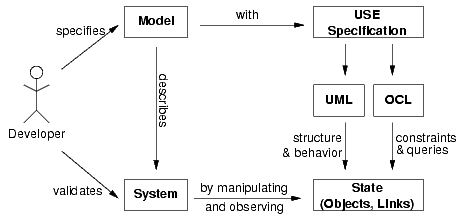
\includegraphics[width=0.8\textwidth]{figures/c1/USE_Overview.png}
    \caption{USE Overview.}
    \label{fig:use_overview}
\end{figure}

\subsection{USE Model Validator}
The Model Validator extends USE's capabilities through a specialized plugin that 
automates the generation of object diagrams from class diagrams within a configurable 
search space \cite{USE}. This plugin bridges the gap between manual model animation 
and systematic verification by employing a transformation-based approach. The 
validator converts UML/OCL models into relational logic using Kodkod, which is 
subsequently transformed into a boolean satisfiability (SAT) problem for efficient 
analysis. When a solution is found, it is immediately displayed as an object diagram 
in the USE interface, with the option to explore alternative valid states. Developers 
control the validation process through configuration files (.properties) that define 
search parameters, including upper and lower bounds for classes, attributes, and 
associations. These configurations can be supplemented with additional OCL invariants 
to target specific scenarios. When executed via the validate command, the Model 
Validator systematically searches for system states that satisfy all constraints, 
reporting either SATISFIABLE (with a corresponding object diagram) when a valid 
configuration exists, or UNSATISFIABLE when the constraints cannot be collectively 
satisfied. This automated approach significantly enhances USE's ability to detect 
inconsistencies and validate model properties that would be difficult to verify 
through manual testing alone.


\subsection{Filmstripping}

\subsubsection{Overview}
Filmstripping is a model transformation technique developed to extend USE's 
verification capabilities from static structure to dynamic behavior \cite{Filmstripping}. 
While standard OCL validation tools (including USE's Model Validator) primarily 
focus on structural aspects like invariants, the filmstrip approach enables 
verification of behavioral properties by transforming dynamic specifications into 
static ones. The method works by converting a UML/OCL model containing both invariants 
and operation pre/postconditions into an equivalent model containing only invariants. 
This transformed "filmstrip model" consists of the original application model 
augmented with specialized structures that capture system state progression. The 
key insight is the introduction of explicit \texttt{Snapshot} classes that represent 
individual system states, with \texttt{OperationCall} classes that connect 
consecutive snapshots. Through this transformation, temporal sequences of operations 
and object states are flattened into a single, verifiable object diagram. Pre and 
postconditions from the original model are systematically converted into invariants 
that constrain relationships between snapshots, effectively embedding behavioral 
specifications within the static structure. This approach enables the Model Validator 
to verify complex behavioral properties—including operation sequencing, state 
transitions, and temporal constraints—using the same validation mechanisms originally 
designed for structural verification. By bridging the gap between static and dynamic 
validation, filmstripping provides a comprehensive framework for verifying both 
aspects of a model within a single technical infrastructure. In the following 
subsection, we detail the specific transformation process that converts standard 
UML/OCL models into filmstrip models, explaining how operation contracts are 
transformed into invariants and how system state progression is represented.

\subsubsection{Filmstrip Model Transformation}

\begin{figure}
    \centering
    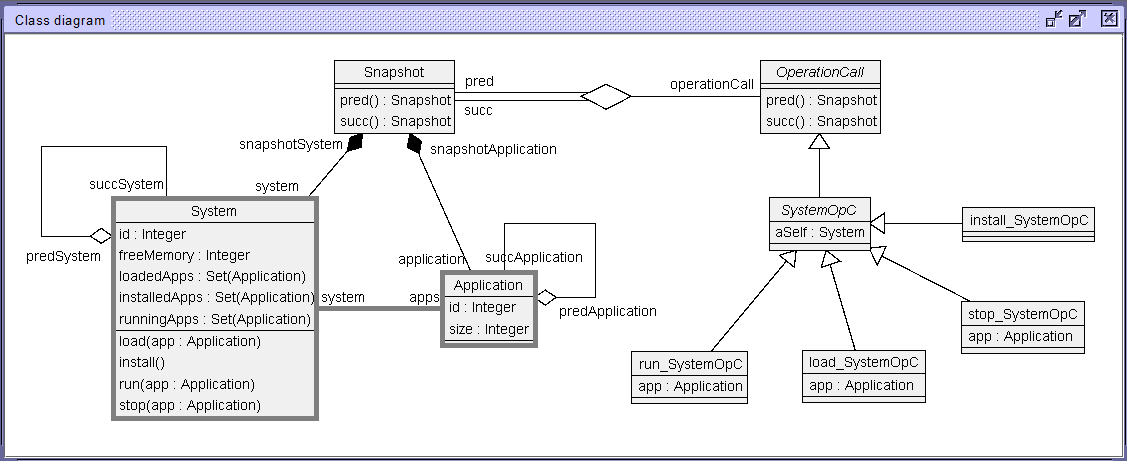
\includegraphics[width=1\textwidth]{figures/c1/SoftwareSystem/SS_Filmstrip_Gray_Edited.png}
    \caption{Filmstrip Model Transformation.}
    \label{fig:filmstrip_model}
\end{figure}

The filmstrip transformation process is best illustrated through an example. 
Figure \ref{fig:filmstrip_model} shows the transformation of our Software System 
model from Figure \ref{fig:class_diagram_software_system} into its filmstrip 
equivalent. The original application model—classes \texttt{System} and 
\texttt{Application} with their \texttt{SystemApplication} association—remains 
intact within the filmstrip model, visually distinguished by gray borders.

The transformation is performed automatically by the Filmstrip Plugin for USE, which 
augments the original model with additional elements (shown without gray borders). 
These elements include \texttt{Snapshot} objects that capture individual system 
states and \texttt{OperationCall} classes (with suffix \texttt{OpC}) that represent 
the operations from the application model. Each operation is converted into a 
corresponding \texttt{OperationCall} class containing attributes for the context 
object (self) and operation parameters.

The complete transformation process involves the following steps \cite{Filmstripping}:
\vspace{-1.2em}
\paragraph{Transformation of classes:} All classes and attributes from the 
application model are preserved in the filmstrip model. Two essential classes are 
added: \texttt{Snapshot}, which associates objects with specific system states, 
and \texttt{OperationCall}, which represents state transitions. Operation parameters 
become attributes in their respective operation call classes, and all operation call 
classes inherit from the base \texttt{OperationCall} class through generalization.
\vspace{-1.2em}
\paragraph{Transformation of associations:} All original associations are maintained 
in the filmstrip model. A crucial ternary association is added to link pre-snapshots 
to post-snapshots through operation calls, representing the system's state evolution. 
Additional associations connect application objects to their respective snapshots, 
ensuring that each object exists in exactly one snapshot state, while aggregation 
links represent object persistence across snapshots.
\vspace{-1.2em}
\paragraph{Transformation of operation definitions and invariants:} Operation 
definitions and invariants from the application model are incorporated without 
modification.
\vspace{-1.2em}
\paragraph{Transformation of pre- and postconditions:} Operation contracts (pre- and 
postconditions) are converted into invariants in the filmstrip model, associated with 
their respective operation call classes. These invariants are evaluated once for each 
operation call instance, preserving the semantic equivalence between the original 
contracts and their filmstrip representations.

\newpage\cleardoublepage
\chapter{Specification and Verification of Temporal Properties in OCL}

\section{Introduction}

\hspace{1cm} OCL provides strong support for structural properties in UML models but 
falls short when specifying dynamic system behavior. Operating only on single states 
or individual transitions, OCL cannot express properties spanning multiple states or 
responding to system events. This limitation is significant for modern systems 
requiring temporal and reactive behaviors.

Temporal logics like LTL and CTL offer formal frameworks for temporal properties but 
require specialized knowledge unfamiliar to most UML designers. This creates a practical 
barrier for practitioners comfortable with UML/OCL but not with formal temporal notations.

This chapter presents two main contributions:

First, we build upon the existing Temporal OCL (TOCL) extension \cite{TOCL}, which already 
incorporates temporal operators like \textit{always}, \textit{sometime}, and 
\textit{until} for reasoning about system evolution over time. However, TOCL remains 
limited in its ability to express event-based properties. Our TOCL+ extension 
addresses this limitation by introducing enhanced event constructs for detecting 
specific system occurrences such as operation calls and state changes, along with 
support for bounded existence properties (e.g., "an operation is called exactly n 
times" or "at most n times"). TOCL+ maintains OCL's familiar syntax while 
significantly expanding its capabilities for specifying event-driven and quantified 
temporal behaviors.
% First, TOCL+ extends OCL with temporal and event capabilities. It adds temporal 
% operators like \textit{always}, \textit{sometime}, and \textit{until} for reasoning 
% about system evolution over time, and introduces event constructs for detecting 
% specific system occurrences such as operation calls and state changes. TOCL+ maintains 
% OCL's familiar syntax while enabling complex dynamic specifications.

Second, we introduce an approach that enables verification of TOCL+ 
specifications using existing tools. This approach transforms UML/OCL models into 
filmstrip models representing state sequences, and translates TOCL+ specifications 
into standard OCL constraints verifiable within these models.

The chapter is organized as follows:
\begin{itemize}
    \item Section 2.2 presents the specification approach.
    
    \item Section 2.3 details the verification approach.
\end{itemize}

Together, these contributions provide a complete solution for both specifying and 
verifying temporal properties within the model-driven engineering paradigm.
\section{An Extended OCL for Temporal and Event Specifications}

%%%%% TOCL
\subsection{TOCL}

\hspace{1cm} In this thesis, we leverage TOCL, as introduced by Ziemann and Gogolla \cite{TOCL}, 
as the temporal foundation for specifying properties that must hold over time across 
multiple states of a system. Standard Object Constraint Language (OCL) is limited to 
evaluating constraints within a single system state or across a single state transition 
(via pre- and postconditions), which is insufficient for capturing the dynamic behaviors 
inherent in many system requirements. For instance, properties such as "eventually, 
the system will reach a stable state" or "once a condition is met, it must remain 
true thereafter" require reasoning over sequences of states. TOCL addresses this limitation 
by extending OCL with elements of linear temporal logic, enabling the expression of such 
temporal properties within a familiar OCL-like syntax.

TOCL's comprehensive set of temporal operators, categorized into future and past 
operators, provides the essential temporal reasoning capabilities for our work. 
In this thesis, we adopt these operators unchanged as the basis for modeling and 
verifying dynamic system behaviors over time. However, to address systems that 
exhibit reactive behaviors driven by specific events, we extend TOCL into TOCL+ 
by integrating novel event-based constructs. This extension, detailed in the next 
section, complements TOCL’s temporal framework, enabling a more holistic specification 
of both state-based temporal properties and event-driven dynamics. Below, we review 
the adopted TOCL temporal operators, their syntax, and semantics, which serve as 
the cornerstone of TOCL+.

%%%
\subsubsection{Adopted TOCL Temporal Operators}
TOCL defines two categories of temporal operators that we adopt in our work:

\paragraph{Future Operators:}
\begin{itemize}
    \item \textbf{next $e$:} True if the expression $e$ holds in the next state.
    \item \textbf{always $e$:} True if $e$ holds in the current state and all subsequent states.
    \item \textbf{sometime $e$:} True if $e$ holds in the current state or at least one future state.
    \item \textbf{always $e_1$ until $e_2$:} True if $e_1$ remains true until $e_2$ becomes true, or if $e_1$ remains true indefinitely if $e_2$ never becomes true.
    \item \textbf{sometime $e_1$ before $e_2$:} True if $e_1$ becomes true at some point before $e_2$ does, or if $e_1$ becomes true and $e_2$ never does.
\end{itemize}

\paragraph{Past Operators:}
\begin{itemize}
    \item \textbf{previous $e$:} True if $e$ was true in the previous state (or if there is no previous state, i.e., at the initial state).
    \item \textbf{alwaysPast $e$:} True if $e$ was true in all past states.
    \item \textbf{sometimePast $e$:} True if $e$ was true in at least one past state.
    \item \textbf{always $e_1$ since $e_2$:} True if $e_1$ has been true since the last time $e_2$ was true.
    \item \textbf{sometime $e_1$ since $e_2$:} True if $e_1$ has been true at some point since the last time $e_2$ was true.
\end{itemize}

For the formal semantics of these operators, we refer to the original work by 
Ziemann and Gogolla \cite{TOCL}, which defines them over sequences of system states.

%%%
\subsubsection{Example Specifications}
To demonstrate the practical application of these operators, we apply them to 
the software system case study introduced in Chapter 1:

%%%%% Event
\subsection{Event Constructs in OCL}

\hspace{1cm} 
% Our approach to event specification adopts the synchronous paradigm, which provides 
% well-founded mathematical semantics and enables formal verification. The essence 
% of this paradigm is the atomicity of reactions (operation calls) where all occurring 
% events during a reaction are considered simultaneous. Under this paradigm, an 
% operation call leads the system directly from a pre-state to a post-state without 
% intermediate states being observable.

To capture these concepts, TOCL+ introduces two primary event constructs:

\begin{itemize}
    \item \textbf{isCalled}: A generic event construct that unifies operation events. It detects when an operation is invoked on an object, representing the atomic transition from a pre-state to a post-state.
    
    \item \textbf{becomesTrue}: A state change event that is parameterized by an OCL boolean expression P. It designates a step in which P becomes true (i.e., P was evaluated to false in the previous state and is true in the current state). In the object-oriented paradigm, a state change is necessarily a consequence of some operation call, therefore becomesTrue acts as syntactic sugar for any operation call that causes P to switch from false to true.
\end{itemize}

\subsubsection{Formal Definition}

Formally, we define events in terms of operations and state transitions. Let O be the set of all operations and E be the set of all OCL boolean expressions in a model. An event is either:

\begin{itemize}
    \item isCalled(op) - representing a call to operation op, optionally with precondition pre and postcondition post
    \item becomesTrue(P) - representing any operation call that transitions the system from a state where ¬P holds to a state where P holds
\end{itemize}

This formal definition enables precise reasoning about when events occur during system execution and forms the foundation for our verification approach.

\subsubsection{Examples}

To illustrate these event constructs, consider a banking system with an Account class:

\begin{itemize}
    \item isCalled(account.withdraw(100)) - Detects when the withdraw operation is called with parameter 100 on an account object
    \item becomesTrue(account.balance < 0) - Detects when an account's balance transitions from non-negative to negative
\end{itemize}

These examples demonstrate how event constructs enable the specification of critical moments in a system's execution, providing the foundation for more complex temporal properties. By combining these event constructs with the temporal operators from TOCL, we create a powerful specification language capable of expressing reactive behaviors and complex temporal patterns.

%%% Sample
% Events are predicates to specify sets of instants within the time line. In Section 1.4.2, we discussed the different types of
% events in the object-oriented approach. There are operation (call/start/end) events, time-triggered events and state change
% events. We have seen that when integrating the clock into the system, time-triggered events are particular state change
% events. Hence, we only need to extend OCL with the necessary construct for both operation and state change events.
% We aim to connect our OCL temporal extension to formal methods such as model-checking and test scenario generation.
% Formal methods are mainly based on the synchronous paradigm that has well-founded mathematical semantics and that
% allows formal verification of the programs and automatic code generation. The essence of the synchronous paradigm is the
% atomicity of reactions (operation calls) where all the occurring events during such a reaction are considered simultaneous.
% In our work, we adopt the synchronous paradigm, and we merge the operation (call/start/end) events into one call event,
% named isCalled, that leads the system from a pre-state to a post-state without considering neither observing intermediate
% change states.
% isCalled: is a generic event construct that unifies both operation events and state change events.
% becomesTrue: is a state change event that is parameterized by an OCL boolean expression P, and designates a step in
%  which P becomes true, i.e. P was evaluated to false in the previous state. In the object-oriented paradigm, a state change
%  is necessarily a consequence of some operation call, therefore the becomesTrue construct is a syntactic sugar and stands for
%  any operation call switching P to true.
% Formal semantics
% A test case is a scenario in which a set of operations is executed in sequence with observations either before or after each
%  operation execution. Since we are interested in test cases generation (see Section 10), we adopt a scenario-based semantics
%  over the synchronous paradigm to formalize our temporal extension. The essence of that paradigm is the atomicity of
%  reactions (operation calls) where all the events occurring during such a reaction are considered as simultaneous. A reaction
%  is one atomic call event, that leads the system directly from a pre-state to a post-state without going through intermediate
%  states.
% We define the set of all atomic events of a given object model as follows:
% Definition6.1 (Alphabetofatomicevents). Let O be the set of all operations and E be the set of all OCL boolean expressions of
%  an object model M.ThealphabetΣM ofatomicevents (abbreviated as Σ in the following) is defined by the set O×E×E.
%  An atomic event e ∈Σ takes the form: e =(op). It stands for a call of the operation op in a context where pre
%  stands for the precondition satisfied in the pre-state and post stands for the postcondition satisfied in the post-state.
%  We now give the formal meaning of the notion of events introduced in our OCL temporal extension.
%  Definition 6.2 (Events). Let Σ be the alphabet of atomic events, O be the set of all operations and E the set of all OCL
%  boolean expressions. An event is either an isCalled(op,pre,post) or a becomesTrue(P) with:
%  isCalled(op,pre,post) = op,pre,post ∈ Σ pre⇒pre, post⇒post and
%  becomesTrue(P) = (op,pre,post) ∈ Σ op∈O, pre⇒¬P, post⇒ P
%  Definition 6.2 calls for the following comments:– An event does not represent a single atomic event, but a specific subset of atomic events. It is intuitively the set of all
%  atomic events in which the operation op is invoked, in a pre-state which implies the expression pre and leading to a
%  post-state which implies the expression post. The set of all events is then defined6 as the set 2Σ;

\section{Verification of TOCL+ Properties}
\section{Summary}\newpage\cleardoublepage
\chapter{Implementation and Experiment}

\section{Introduction}

\hspace{1cm} In the previous chapter, we introduced TOCL+, an extension of OCL with temporal operators and event constructs, and presented a theoretical framework for specifying and verifying temporal properties in UML models. While the formal semantics and verification approach provide a solid foundation, they require practical tool support to be effectively applied. This chapter bridges the gap between theory and practice by presenting our implementation of a TOCL+ plugin for the USE tool and demonstrating its effectiveness through a detailed case study.

The primary objective of this chapter is twofold. First, we describe the implementation of our TOCL+ plugin for the USE tool, which enables modelers to specify temporal properties using our extended language and automatically verify them using the filmstrip approach. Second, we demonstrate the practical application of TOCL+ through a detailed case study of the Software System model introduced in Chapter 2, showcasing how various types of temporal properties can be effectively specified and verified.

In the following sections, we present the architecture and implementation of our plugin, focusing on how it integrates with the USE tool environment and implements the transformation process described in Chapter 2. We then explore the Software System case study, illustrating how our approach handles the specification and verification of different types of temporal properties in practice.
\section{TOCL+ Tool Support and Implementation}

\subsection{Support tool architecture}

\begin{figure}
    \centering
    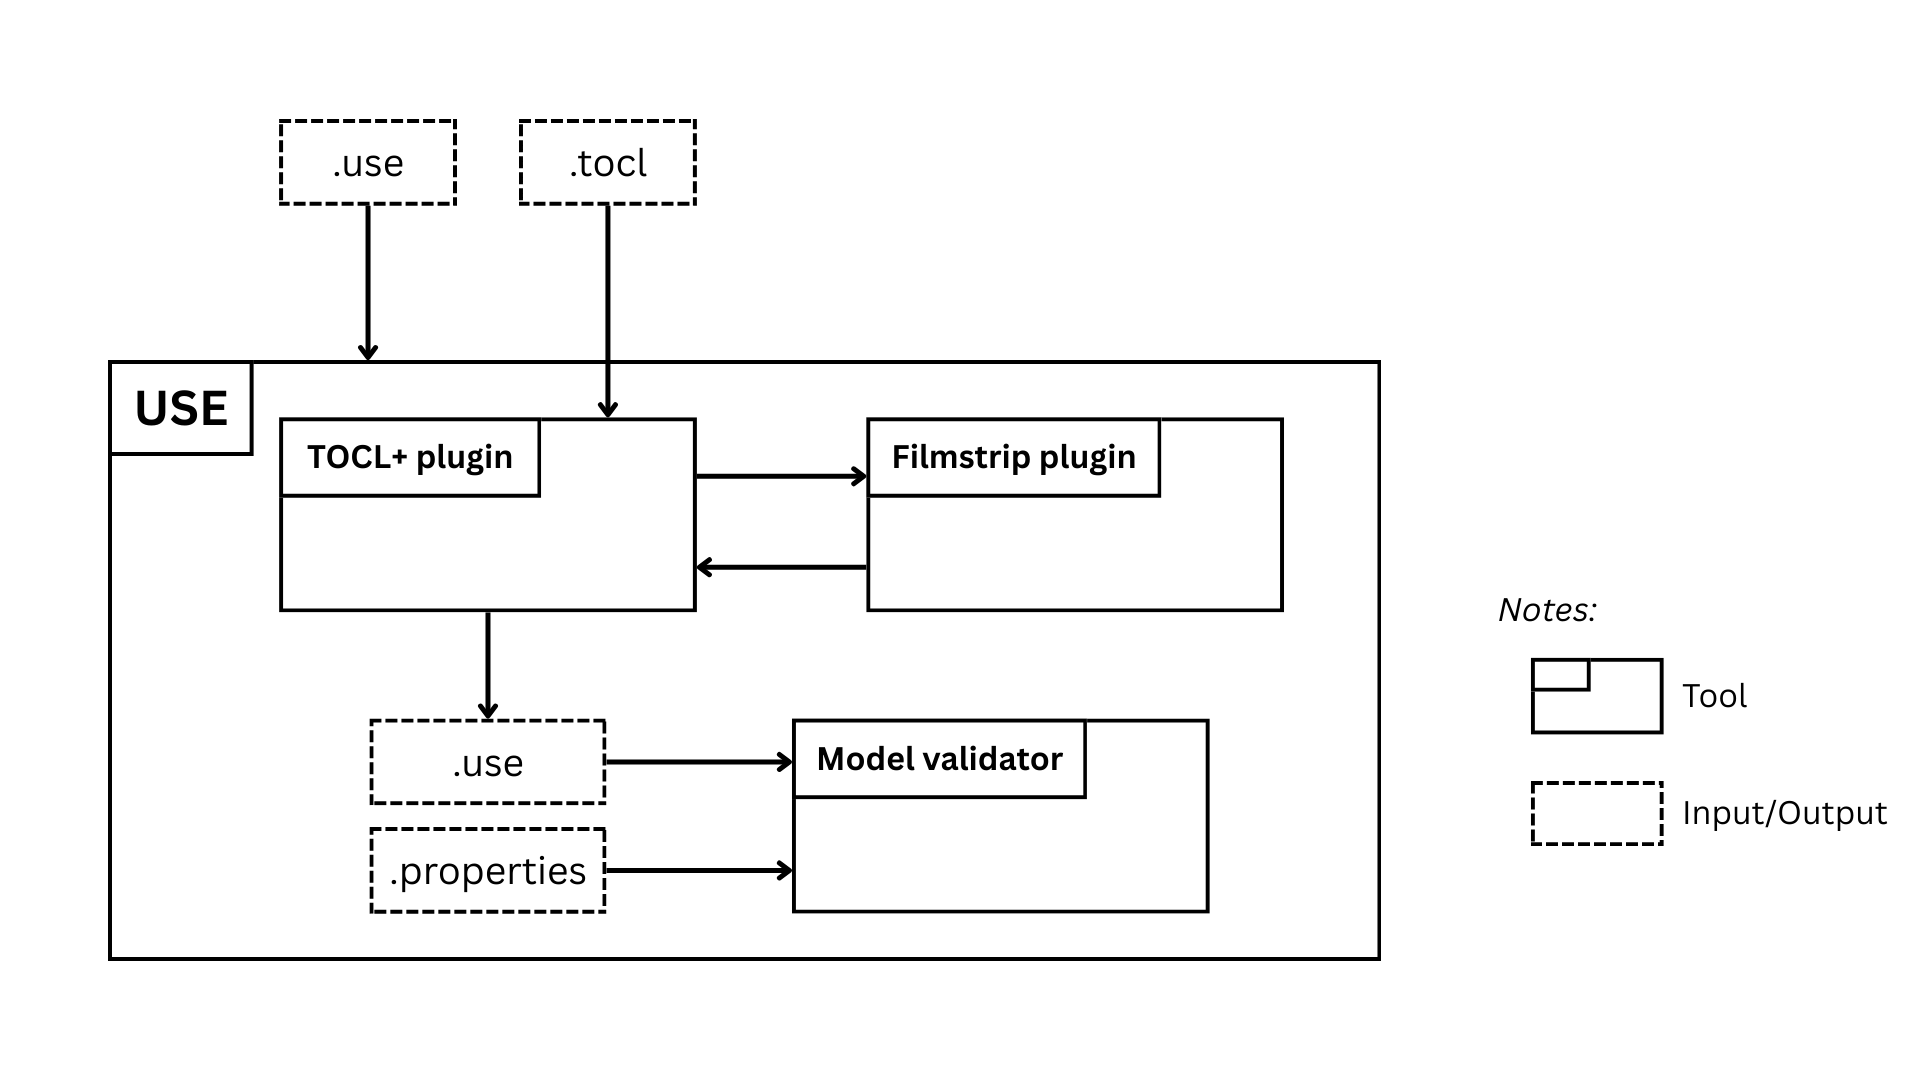
\includegraphics[width=1\textwidth]{figures/c3/Architecture_overview.png}
    \caption{Support Tool Architecture and Verification Workflow.}
    \label{sec:plugin_support_tool_architecture}
\end{figure}

\hspace{1cm} Figure \ref{sec:plugin_support_tool_architecture} illustrates the 
architecture and workflow of our TOCL+ support tool. This integrated verification 
framework combines several components: the existing USE environment, the Filmstrip 
plugin, our TOCL+ plugin, and the Model Validator. The architecture maintains a 
clear separation between modeling, specification, and verification concerns while 
providing a cohesive workflow for users.

The verification process consists of five distinct steps, beginning with preparation 
and ending with validation. First, the user prepares two input files: a standard 
\texttt{.use} file containing the UML/OCL application model and a \texttt{.tocl} 
file containing TOCL+ property specifications. Second, the user loads the application 
model into USE to make it available for transformation. Third, the user activates 
our plugin through the USE interface, selecting both a destination path for the 
output model and the \texttt{.tocl} file containing the temporal properties to verify.

Internally, the plugin then executes a two-phase transformation process. In the 
first phase, it invokes the Filmstrip plugin to transform the application model 
into a filmstrip model following the rules described in Section~\ref{subsec:filmstripping}. 
In the second phase, it processes the TOCL+ expressions using our ANTLR4-generated 
parser and listener components, which implement the transformation rules for 
converting temporal specifications into equivalent OCL constraints. These generated 
constraints are added to the list of invariants in the output model file alongside 
the filmstrip model elements.

To complete the verification process, the user loads this output model back into 
USE together with a configuration file that establishes search bounds, and then 
employs the Model Validator to analyze the constraints. The validator systematically 
explores the search space, determining whether the temporal properties are satisfied 
and providing a model instance as evidence when applicable.

Our primary contribution in this architecture is the TOCL+ plugin, specifically 
the TOCL+ to OCL transformation component that enables the verification of temporal 
properties using existing OCL tools. The implementation details of this transformation 
process, including the translation rules for different temporal operators and event 
constructs, are presented in the next subsection.

\subsection{Implementation of TOCL+ to OCL Transformation}

\hspace{1cm} The core of our contribution lies in the transformation of TOCL+ 
expressions into equivalent OCL constraints that can be verified over filmstrip 
models. This transformation process involves systematically mapping temporal operators 
and event constructs to structural navigations through snapshots and operation calls. 
In this section, we describe our implementation approach and the key translation 
patterns we developed.

Our transformation approach is inspired by the work of \cite{TOCL2OCL}, who 
transformed TOCL \cite{TOCL} into OCL in the context of a Snapshot-Transition Model 
(STM). While their approach also converts temporal properties into static ones, we 
adapted and extended it to work within the filmstrip model context.

To transform TOCL+ expressions, we defined translations for TOCL+ operators and 
events to OCL, as shown in Table \ref{tab:TOCL2OCL}. To create these translations, 
we utilized several query operations provided by the filmstrip structure. 
The self.snapshot query accesses the snapshot associated with an object in the 
"current state" where the expression is being evaluated. The pred() and succ() 
operations, when applied to a snapshot, navigate to the previous and next state 
respectively. For objects to navigate to their corresponding versions in adjacent 
states, we use the two associations .pred and .succ. These navigation mechanisms 
form the foundation for implementing our temporal operator translations.

Note that filmstrip model does not inherently provide any means to identify the same 
logical object across different states - it only provides the .pred and .succ 
associations to navigate between corresponding objects in adjacent snapshots. 
In order to overcome this limitation, we require modelers to add an id attribute 
to all classes in the application model. As seen in Figure \ref{fig:object_diagram_liveness}, 
this allows us to identify the same logical object across different snapshots. 
Internally, when the TOCL+ plugin transforms the model, we add additional 
constraints to ensure this id remains consistent between different states. 
This id attribute is critical in the OCL translation, particularly for event 
constructs like becomesTrue. When navigating with expressions like 
self.snapshot.pred().[ContextObject], we get a collection of objects of the same 
type, and we select the one with matching identity using ->any(o | o.id = self.id).

Table \ref{tab:TOCL2OCL} presents the complete set of translation patterns we 
developed for TOCL+ operators and event constructs. Each pattern systematically 
maps a TOCL+ construct to an equivalent OCL expression interpreted over the filmstrip 
model. The patterns use placeholders (indicated by square brackets) that get 
substituted during the transformation process: \texttt{[s |= P]} indicates that 
property P holds in snapshot s; \texttt{[ContextSnapshot]} is the snapshot in which 
the property is evaluated; \texttt{[ContextObject]} is the object on which the 
property is evaluated; and \texttt{[OpClassName]} is the class representing an 
operation call in the filmstrip model. When applying these patterns, each placeholder 
is replaced with the appropriate expression based on the model context. For example, 
in the liveness property translation shown in Listing \ref{lst:ocl_liveness}, the 
\texttt{[ContextSnapshot]} is replaced with the local variable \texttt{s} inside the 
\texttt{exists} query. The bounded quantifiers (e.g., \texttt{at most}, \texttt{at least}) 
are translated into corresponding comparators (\texttt{<=}, \texttt{>=}). 
The bounded quantifiers in TOCL+ expressions are systematically translated into their 
corresponding OCL comparators: \texttt{at most} becomes less than or equal to 
(\texttt{<=}), while \texttt{at least} becomes greater than or equal to (\texttt{>=}). 
For bounded existence properties without an explicit quantifier (e.g., 
\texttt{isCalled(Op()) 3 times}), the translation applies the equality operator 
(\texttt{=}), enforcing that the event occurs exactly the specified number of times. 
In contrast, when dealing with unbounded event expressions without quantifiers (e.g., 
simply \texttt{isCalled(Op())}), the translation converts the \texttt{select} operation 
into an \texttt{exists} operation, requiring only that the event occurs at least once 
rather than counting occurrences.
    
We implemented the transformation using ANTLR4, a parser generator that creates a 
parse tree from TOCL+ expressions. After defining the translation patterns shown 
in Table \ref{tab:TOCL2OCL}, we created Java listener classes that extend the 
generated parser listeners. The transformation process employs these listener 
components to traverse the parse tree and produce corresponding OCL expressions 
by overriding the generated listener methods. As the parser walks through each node 
in the parse tree, our listeners intercept parse tree events and apply the appropriate 
translation rules, constructing equivalent OCL constraints that navigate through 
the filmstrip structure. The transformation follows a consistent pattern: when a 
temporal operator or event construct is encountered, the listener extracts relevant 
information from the parse tree nodes, applies the corresponding translation pattern, 
and builds the equivalent OCL expression. Our implementation maintains a stack of 
expressions to handle nested structures, pushing both the original TOCL+ expression 
and its OCL translation for later integration into the output model.
Listing \ref{lst:becomesTrue_translation} provides an example of this process for 
the \texttt{becomesTrue} event construct, showing how we extract the expression 
to be evaluated, establish the necessary context, and construct the translated OCL 
expression. 

After processing all the nodes in the parse tree, our implementation finalizes the 
translation in the root node visit. Since TOCL+ is an extension of OCL, many 
constructs remain unchanged and are directly preserved during translation. The 
completion process begins by accessing the token stream to retrieve the complete 
original expression text. Our implementation then systematically pops each translated 
OCL fragment and its corresponding original TOCL+ expression from the stack. Using 
string replacement operations, it substitutes each temporal construct with its 
equivalent OCL translation while preserving the structure of the original expression. 
This approach allows us to handle nested temporal operators naturally, as inner 
expressions are processed before their containing expressions. The final translated 
OCL constraint is then attached to the root of the parse tree and ultimately added 
to the output model as an invariant. This complete process ensures that complex 
temporal properties are accurately transformed into standard OCL constraints that 
can be verified by the Model Validator.

\begin{lstlisting}[
    style=javastyle,
    caption={Translation of becomesTrue event to OCL.},
    label={lst:becomesTrue_translation}
]
TokenStream tokens = parser.getTokenStream();
String originalEvent = tokens.getText(ctx);
String translatedEvent;
// P
String expressionToSatisfy = getOCL(ctx.getChild(2)); 
// e.g., "system", "application"
String roleName = toLowerFirstChar(currentContext); 
String currentSnapshot = "self.snapshot"; 
String selectObject = "->any(o | o.id = self.id)";

// e.g. self.snapshot.system->any(o | o.id = self.id)
String objectAtCurrentSnapshot = currentSnapshot + "." + roleName + selectObject;
String objectAtPreviousSnapshot = currentSnapshot + ".pred()." + roleName + selectObject;
String P_at_currentSnapshot = expressionToSatisfy.replace("self", "currentObject");
String P_at_previousSnapshot = expressionToSatisfy.replace("self", "previousObject");

translatedEvent = 
"let currentObject = " + objectAtCurrentSnapshot +
" in let previousObject = " + objectAtPreviousSnapshot +
" in not (" + P_at_previousSnapshot + ") and (" + P_at_currentSnapshot + ")";

eventStack.push(translatedEvent);
eventStack.push(originalEvent);    
\end{lstlisting}

\begin{longtable}{|>{\footnotesize}p{0.6cm}|>{\scriptsize\raggedright\arraybackslash}p{4cm}|>{\scriptsize\raggedright\arraybackslash}p{\dimexpr\textwidth-4.6cm-4\tabcolsep-3\arrayrulewidth\relax}|}
    \caption{Translation of TOCL+ operators and events to OCL.}
    \label{tab:TOCL2OCL} \\
    \hline
    \textbf{No.} & \textbf{TOCL+} & \textbf{OCL Translation} \\
    \hline
    1 & 
    next P &
    let nextSnapshot:Snapshot = self.snapshot.succ() in [nextSnapshot |= P] \\
    \hline
    2 &
    always P &
    let CS:Snapshot = self.snapshot in Set\{CS\}->closure(s | s.succ())->forAll(s | [s |= P]) \\
    \hline  
    3 &
    always P until Q &
    let CS:Snapshot = self.snapshot
    in let FS:Set(Snapshot) = Set\{CS.succ()\}->closure(s | s.succ())
    in let AllFSQ:Set(Snapshot) = FS->select(s | [s |= Q])
    in let FSQ:Snapshot = AllFSQ->any(s | Set\{s\}->closure(s | s.succ())->includesAll(AllFSQ))
    in let afterQ:Set(Snapshot) = Set\{FSQ\}->closure(s | s.succ())
    in let FSP:Set(Snapshot) = FS->select(s | [s |= P])
    in if FSQ.isDefined() then (if (FSP->size() > 0) then (FS-afterQ = FSP-afterQ) else false endif) else (FS = FSP) endif \\
    \hline
    4 &
    always P since Q &
    let CS:Snapshot = self.snapshot
    in let PS:Set(Snapshot) = Set\{CS.pred()\}->closure(s | s.pred())
    in let AllPSQ:Set(Snapshot) = PS->select(s | [s |= Q])
    in let PSQ:Snapshot = AllPSQ->any(s | Set\{s\}->closure(s | s.pred())->includesAll(AllPSQ))
    in let beforeQ:Set(Snapshot) = Set\{PSQ\}->closure(s | s.pred())
    in let PSP:Set(Snapshot) = PS->including(CS)->select(s | [s |= P])
    in if PSQ.isDefined() then (if (PSP->size() > 0) then (PS->including(CS)-beforeQ = PSP-beforeQ) else false endif) else (PSP = PS->including(CS)) endif \\
    \hline
    5 &
    sometime P &
    let CS:Snapshot = self.snapshot in Set\{CS\}->closure(s | s.succ())->exists(s | [s |= P]) \\
    \hline
    6 &
    sometime P before Q &
    let FS:Set(Snapshot) = Set\{self.snapshot\}->closure(s | s.succ())
    in let PreS:Set(Snapshot) = Set\{self.snapshot.pred()\}->closure(s | s.pred())
    in let AllFSQ:Set(Snapshot) = FS->select(s | [s |= Q])
    in let FSQ:Snapshot = AllFSQ->any(s | Set\{s\}->closure(s | s.succ())->includesAll(AllFSQ))
    in let FSP:Set(Snapshot) = FS->select(s | [s |= P])
    in if FSQ.isDefined() then (if (FSP->size() > 0) then ((Set\{FSQ.pred()\}->closure(s | s.pred())-PreS)->exists(s\_1 | FSP->includes(s\_1))) else false endif) else false endif \\
    \hline
    7 &
    sometime P since Q &
    let CS:Snapshot = self.snapshot
    in let PS:Set(Snapshot) = Set\{CS.pred()\}->closure(s | s.pred())
    in let AllPSQ:Set(Snapshot) = PS->select(s | [s |= Q])
    in let PSQ:Snapshot = AllPSQ->any(s | Set\{s\}->closure(s | s.pred())->includesAll(AllPSQ))
    in let PSP:Set(Snapshot) = PS->select(s | [s |= P])
    in if PSQ.isDefined() then (Set{PSQ}->closure(s | s.succ())->excluding(null)->intersection(PS)->exists(s | PSP->includes(s))) else false endif \\ 
    \hline
    8 &
    previous P &
    let previousSnapshot:Snapshot = self.snapshot.pred() in [previousSnapshot |= P] \\
    \hline
    9 &
    sometimePast P &
    let CS:Snapshot = self.snapshot in Set\{CS.pred()\}->closure(s | s.pred())->exists(s | [s |= P]) \\
    \hline
    10 &
    alwaysPast P &
    let CS:Snapshot = self.snapshot in Set\{CS.pred()\}->closure(s | s.pred())->forAll(s | [s |= P]) \\
    \hline
    11 &
    isCalled(Op()) &
    [OpClassName].allInstances()->exists(op | op.succ() = [ContextSnapshot]) \\
    \hline
    12 &
    isCalled(Op($param_1$, $\ldots$, $param_n$)) &
    [OpClassName].allInstances()->exists(op | op.succ() = [ContextSnapshot] and
    (Set\{op.$param_1$.succ\}->closure(p | p.succ)->includes($param_1$) or Set\{op.$param_1$.pred\}->closure(p | p.pred)->includes($param_1$))
    and ($\ldots$)
    and (Set\{op.$param_n$.succ\}->closure(p | p.succ)->includes($param_n$) or Set\{op.$param_n$.pred\}->closure(p | p.pred)->includes($param_n$))) \\
    \hline
    13 &
    isCalled(Op()) [at most | at least | ] n times &
    [OpClassName].allInstances()->select(op | op.succ() = [ContextSnapshot])->size() [<= | >= | =] n \\
    \hline
    14 &
    isCalled(Op($param_1$, $\ldots$, $param_n$)) [at most | at least | ] n times &
    [OpClassName].allInstances()->select(op | op.succ() = [ContextSnapshot] and
    (Set\{op.$param_1$.succ\}->closure(p | p.succ)->includes($param_1$) or Set\{op.$param_1$.pred\}->closure(p | p.pred)->includes($param_1$)) 
    and ($\ldots$) 
    and (Set\{op.$param_n$.succ\}->closure(p | p.succ)->includes($param_n$) or Set\{op.$param_n$.pred\}->closure(p | p.pred)->includes($param_n$)))->size() [<= | >= | =] n \\
    \hline
    15 &
    becomesTrue(P) &
    let currentObject = self.snapshot.[ContextObject]->any(o | o.id = self.id) in
    let previousObject = self.snapshot.pred().[ContextObject]->any(o | o.id = self.id) in 
    not [previousObject |= P] and [currentObject |= P] \\
    \hline
\end{longtable}

\section{Case study: Software System model}
\label{sec:case_study_software_system}

\subsection{Model Specification}

The Software System model shown in Listing \ref{lst:software_system_specification} 
is the same model introduced in Chapter 1 to demonstrate OCL constraints (see 
Figure \ref{fig:class_diagram_software_system}). As a reminder, this model represents 
a simplified operating system that manages applications through their lifecycle. 
It consists of two main classes: \texttt{System} and \texttt{Application}, connected 
through an association. The \texttt{System} maintains three collections 
(\texttt{loadedApps}, \texttt{installedApps}, and \texttt{runningApps}) representing 
different application states, and provides four operations to manage applications: 
\texttt{load}, \texttt{install}, \texttt{run}, and \texttt{stop}.

The \texttt{freeMemory} attribute represents available disk space, which decreases 
when applications are loaded. The \texttt{load} operation acts as a download action, 
reducing available memory when an application is acquired. The \texttt{install} 
operation processes all loaded applications at once, moving them from 
\texttt{loadedApps} to \texttt{installedApps}. When an application is running, it 
exists in both the \texttt{installedApps} and \texttt{runningApps} sets simultaneously. 
The \texttt{SystemApplication} association facilitates navigation between system and 
applications in this simplified model.

Note that the numerous postconditions like \texttt{sameInstalledAndRunning}, 
\texttt{sameRunning}, \texttt{sameMemory}, \texttt{sameLoaded}, \texttt{sameInstalled}, 
and the \texttt{unchanged} constraints serve as helper constraints in the verification 
context: since the Model Validator assigns random values to attributes when exploring 
possible states, these constraints ensure that attributes unaffected by an operation 
remain consistent between snapshots.

This model serves as an ideal case study for temporal property verification as it 
involves operations with clear sequential dependencies and state transitions that 
cannot be adequately expressed using standard OCL. The full specification below 
includes all constraints and operation contracts necessary for our verification 
experiments.

\begin{lstlisting}[
    caption={Specification of the Software System model in USE environment.},
    label={lst:software_system_specification}
]
model SoftwareSystem
-- Classes
class System
attributes
    id : Integer
    freeMemory : Integer init = 10
    loadedApps : Set(Application) init = Set{}
    installedApps : Set(Application) init = Set{}
    runningApps : Set(Application) init = Set{}
operations
    load(app : Application)
    begin
        self.loadedApps := self.loadedApps->including(app);
        self.freeMemory := self.freeMemory - app.size;
    end
    install()
    begin
        self.installedApps := self.installedApps->union(self.loadedApps);
        self.loadedApps := self.loadedApps->reject(true)->excluding(null);
    end
    run(app : Application)
    begin
        self.runningApps := self.runningApps->including(app);
    end
    stop(app : Application)
    begin
        self.runningApps := self.runningApps->excluding(app);
    end
end
class Application
attributes
    id : Integer
    size : Integer
end
-- Associations
association SystemApplication between
    System[1] role system
    Application[0..*] role apps
end
-- Invariants
constraints
context System
    inv memoryConstraint: self.freeMemory >= 0
    inv notLoadedAndInstalled: self.loadedApps->intersection(self.installedApps)->isEmpty()
    inv sets: let appNumber: Integer = self.apps->size() in
        (self.loadedApps->size() <= appNumber and
        self.installedApps->size() <= appNumber and
        self.runningApps->size() <= appNumber)
    inv notContainsNull:
        not self.loadedApps->includes(null) and
        not self.installedApps->includes(null) and
        not self.runningApps->includes(null)

context Application
    inv sizeConstraint: self.size > 0

context System::load(app: Application)
    pre notLoaded: not self.loadedApps->includes(app) and
                    not self.installedApps->includes(app) and
                    not self.runningApps->includes(app)
    pre enoughMemory: self.freeMemory >= app.size
    post loaded: self.loadedApps = self.loadedApps@pre->including(app)
    post freeMemory: self.freeMemory = self.freeMemory@pre - app.size
    post unchanged:
        self.apps->forAll(app |
            app.size = app.size@pre and
            app.id = app.id@pre)
    post sameInstalledAndRunning:
        self.installedApps = self.installedApps@pre and
        self.runningApps = self.runningApps@pre

context System::install()
    pre hasLoadedApps: self.loadedApps->notEmpty()
    post installed: self.installedApps = self.installedApps@pre->union(self.loadedApps@pre)
    post loadedAppsEmpty: self.loadedApps = self.loadedApps@pre->reject(true)->excluding(null)
    post sameRunning: self.runningApps = self.runningApps@pre
    post sameMemory: self.freeMemory = self.freeMemory@pre
    post unchanged:
        self.apps->forAll(app |
            app.size = app.size@pre and
            app.id = app.id@pre)

context System::run(app : Application)
    pre isInstalled: self.installedApps->includes(app)
    pre notRunning: not self.runningApps->includes(app)
    post running: self.runningApps = self.runningApps@pre->including(app)
    post sameLoaded: self.loadedApps = self.loadedApps@pre
    post sameInstalled: self.installedApps = self.installedApps@pre
    post sameMemory: self.freeMemory = self.freeMemory@pre
    post unchanged:
        self.apps->forAll(app |
            app.size = app.size@pre and
            app.id = app.id@pre)

context System::stop(app : Application)
    pre isRunning: self.runningApps->includes(app)
            and self.installedApps->includes(app)
    post notRunning: self.runningApps = self.runningApps@pre->excluding(app)
    post sameInstalled: self.installedApps = self.installedApps@pre
    post sameLoaded: self.loadedApps = self.loadedApps@pre
    post sameMemory: self.freeMemory = self.freeMemory@pre
    post unchanged:
        self.apps->forAll(app |
            app.size = app.size@pre and
            app.id = app.id@pre)
\end{lstlisting}


\subsection{Temporal Property Verification}
% For each of the 4 properties:
%   1. Brief description of what the property verifies
%   2. TOCL+ specification
%   3. Generated OCL translation
%   4. Verification results

% The TOCL+ temporal properties for the Software System model were shown in Listing 
% \ref{lst:tocl+}. And Listing \ref{lst:ocl_translations} shows the OCL translations 
% for those TOCL+ properties. 

To demonstrate our TOCL+ to OCL transformation approach, we verified four temporal 
properties from Chapter 2 against the Software System model: safety1 (applications 
must be loaded before being run), safety2 (applications must follow the 
load-install-run sequence), safety3 (applications are loaded at most once), and 
liveness (loaded applications will eventually be installed). Listing 
\ref{lst:ocl_translations} shows the OCL constraints generated by our transformation 
plugin for these properties. While the resulting OCL expressions are considerably 
more complex than their TOCL+ counterparts—involving extensive navigation through 
the filmstrip model—they correctly implement the required temporal semantics. This 
demonstrates how our approach enables temporal reasoning within standard OCL, 
shielding modelers from the underlying complexity.

\begin{lstlisting}[
    caption={OCL Translations for TOCL+ properties shown in listing \ref{lst:tocl+}.},
    label={lst:ocl_translations}
]
context System
inv safety1:
    self.runningApps->notEmpty() implies
    self.runningApps->forAll(app |
        (run_SystemOpC.allInstances()->exists(op | op.succ() = self.snapshotSystem and (Set{op.app.succApplication}->closure(p | p.succApplication)->includes(app) or Set{op.app.predApplication}->closure(p | p.predApplication)->includes(app)))) implies
        (let CS:Snapshot = self.snapshotSystem in Set{CS.pred()}->closure(s | s.pred())->exists(s | (load_SystemOpC.allInstances()->exists(op | op.succ() = s and (Set{op.app.succApplication}->closure(p | p.succApplication)->includes(app) or Set{op.app.predApplication}->closure(p | p.predApplication)->includes(app))))))
    )

context System
inv safety2:
    self.runningApps->notEmpty() implies
    self.runningApps->forAll(app |
        (run_SystemOpC.allInstances()->exists(op | op.succ() = self.snapshotSystem and (Set{op.app.succApplication}->closure(p | p.succApplication)->includes(app) or Set{op.app.predApplication}->closure(p | p.predApplication)->includes(app)))) implies
        (let CS:Snapshot = self.snapshotSystem in let PS:Set(Snapshot) = Set{CS.pred()}->closure(s | s.pred())->excluding(null) in let AllPSQ:Set(Snapshot) = PS->select(s | (load_SystemOpC.allInstances()->exists(op | op.succ() = s and (Set{op.app.succApplication}->closure(p | p.succApplication)->includes(app) or Set{op.app.predApplication}->closure(p | p.predApplication)->includes(app))))) in let PSQ:Snapshot = AllPSQ->any(s | Set{s}->closure(s | s.pred())->includesAll(AllPSQ)) in let PSP:Set(Snapshot) = PS->select(s | install_SystemOpC.allInstances()->exists(op | op.succ() = s)) in if PSQ.isDefined() then (Set{PSQ}->closure(s | s.succ())->excluding(null)->intersection(PS)->exists(s | PSP->includes(s))) else false endif)
    )

context System
inv safety3:
    self.installedApps->notEmpty() implies
    self.installedApps->forAll(app |
        (let CS:Snapshot = self.snapshotSystem in Set{CS.pred()}->closure(s | s.pred())->exists(s | (load_SystemOpC.allInstances()->select(op | op.succ() = s and (Set{op.app.succApplication}->closure(p | p.succApplication)->includes(app) or Set{op.app.predApplication}->closure(p | p.predApplication)->includes(app)))->size() <= 1)))
    )

context System
inv liveness:
    self.loadedApps->notEmpty() implies
    self.loadedApps->forAll(app |
        (let CS:Snapshot = self.snapshotSystem in Set{CS}->closure(s | s.succ())->excluding(null)->exists(s | install_SystemOpC.allInstances()->exists(op | op.succ() = s)))
    )
\end{lstlisting}


\subsection{Analysis of Results}
% Figure \ref{fig:object_diagram_case_study} shows a scenario generated by the USE Model
% Validator. The scenario represents a system execution path start with loading an 
% application, installing it, running it, and stopping it. The OCL result for this
% scenario is shown in Figure \ref{fig:ocl_result_case_study}. 

\hspace{1cm} Figure \ref{fig:object_diagram_case_study} shows a concrete scenario 
generated by the USE Model Validator when verifying our temporal properties. This 
scenario visualizes a complete application lifecycle through the software system, 
illustrating a sequence of operation calls: loading an application, installing it, 
running it, and finally stopping it. This execution path is particularly valuable 
as it exercises all four operations of our model in their expected sequence.

As shown in Figure \ref{fig:ocl_result_case_study}, all temporal properties are 
satisfied in this scenario. Each property verification confirms an important aspect 
of our system's behavior: safety1 verifies that the application was indeed loaded 
before being run; safety2 confirms the correct operational sequence was followed 
(load→install→run); safety3 validates that the application was loaded exactly once; 
and the liveness property confirms that after being loaded, the application was 
eventually installed.

These results demonstrate two important aspects of our approach. First, they validate 
the correctness of our transformation rules by confirming that the generated OCL 
constraints accurately encode the intended temporal semantics. Despite their 
complexity, the translated constraints correctly identify valid execution paths. 
Second, they show how our approach supports automated verification of complex 
temporal properties that would be impossible to express in standard OCL.

\begin{figure}
    \centering
    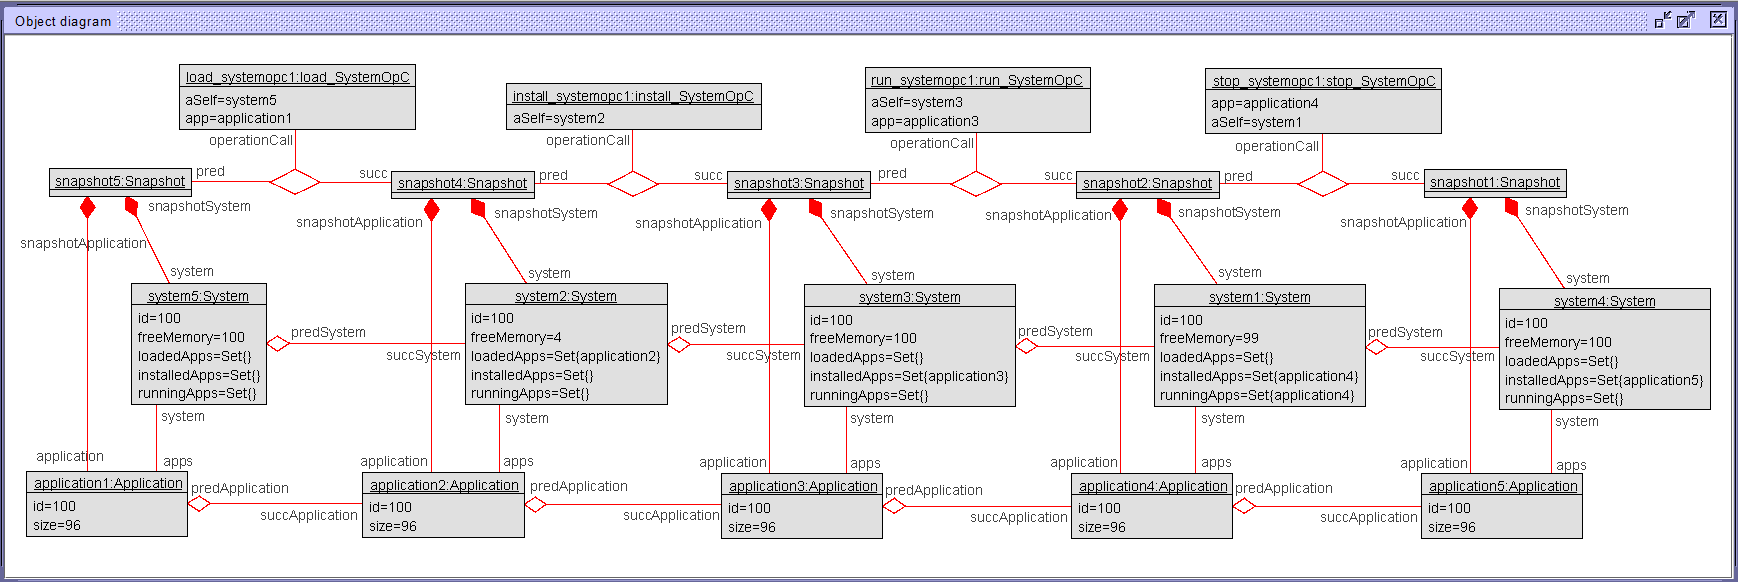
\includegraphics[width=1\textwidth]{figures/c3/CaseStudy_ObjectDiagram.png}
    \caption{A scenario generated by the USE Model Validator.}
    \label{fig:object_diagram_case_study}
\end{figure}

\begin{figure}
    \centering
    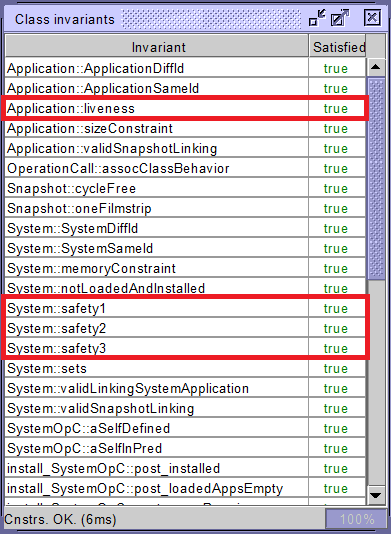
\includegraphics[width=0.4\textwidth]{figures/c3/OCL_result_full_edited.png}
    \caption{OCL result for generated scenario \ref{fig:object_diagram_case_study}.}
    \label{fig:ocl_result_case_study}
\end{figure}
\section{Discussion}

\hspace{1cm} Our TOCL+ approach for specifying and verifying temporal properties in 
UML/OCL models offers several advantages over existing approaches but also comes with 
certain limitations that warrant discussion.

The primary strength of our approach lies in its integration with standard modeling 
environments and tools. By extending OCL rather than introducing an entirely new 
formalism, we maintain compatibility with existing modeling practices while adding 
temporal verification capabilities. This integration allows modelers to work within 
familiar environments while gaining the ability to verify a broader class of 
properties. Our transformation-based approach also offers considerable flexibility. 
By converting TOCL+ specifications to standard OCL constraints on filmstrip models, 
we leverage established OCL tool capabilities without requiring specialized temporal 
verification engines. This provides a pragmatic solution that can be adopted without 
significant infrastructure changes or learning costs. The event-based constructs in 
TOCL+ address a significant gap in existing temporal OCL extensions. While previous 
approaches like TOCL provide temporal operators, they lack robust support for event 
detection and bounded existence properties. Our extensions make it possible to express 
important constraints related to operation calls and state changes, significantly 
broadening the range of verifiable properties.

While effective in practice, our approach has several technical limitations. The OCL 
constraints generated by our transformation can be complex, potentially affecting 
verification performance for large models with numerous temporal properties. These 
constraints involve intricate navigation through snapshots and careful handling of 
object identity, which may impact scalability for very large systems. Our approach 
also requires modelers to add identifier attributes to domain classes to maintain 
object identity across snapshots. This requirement introduces a small burden on 
modelers and slightly modifies the original domain model. A more elegant solution 
would be to handle object identity tracking automatically within the transformation 
framework. The current implementation also has limited support for complex expressions 
within event specifications. For example, nested event expressions or complex guards 
on events might not translate correctly in all cases. This restricts the sophistication 
of temporal properties that can be reliably verified.

From a methodological perspective, our work lacks a formal definition of the TOCL+ 
language and its transformation to OCL. Although our patterns appear to work correctly 
based on empirical evidence from case studies, we haven't provided formal proofs of 
semantic preservation between TOCL+ expressions and their OCL translations. This 
represents a theoretical gap that could affect confidence in the correctness of 
verification results for complex scenarios. Additionally, while our approach handles 
the core temporal operators and event constructs well, it doesn't yet support 
probabilistic or real-time properties. Systems with strict timing requirements or 
probabilistic behavior patterns would require extensions beyond the current 
capabilities.

Several promising research directions emerge from these limitations. The development 
of optimization techniques for the generated OCL constraints could significantly 
improve verification performance. Extending the approach with quantitative time 
constraints would enable verification of real-time properties. Creating a pattern 
library of common temporal verification scenarios with optimized translations would 
make the approach more accessible to practitioners. Enhancing the plugin with more 
intuitive visualizations of counterexamples when temporal properties are violated 
would improve usability. The formal definition of TOCL+ semantics and transformation 
rules, along with mathematical proofs of their correctness, would strengthen the 
theoretical foundations of the approach and provide stronger guarantees about 
verification results.
\section{Summary}
\hspace{1cm} In this chapter, we presented the practical implementation of our TOCL+ 
approach through a plugin for the USE tool and demonstrated its effectiveness through 
a detailed case study. The implementation bridges the gap between the theoretical 
foundations established in Chapter 2 and practical model verification by enabling 
modelers to specify temporal properties in a high-level language while leveraging 
existing OCL verification tools. Our plugin successfully implements the transformation 
rules that convert TOCL+ expressions into equivalent OCL constraints interpreted 
over filmstrip models. The implementation uses ANTLR4 for parsing TOCL+ expressions 
and employs a listener-based approach to systematically translate temporal operators 
and event constructs into structural OCL navigations.

The Software System case study demonstrated how our approach enables verification 
of diverse temporal properties that would be impractical to express in standard OCL. 
The safety properties successfully enforced correct operational sequencing and 
uniqueness constraints, while the liveness property verified eventual progress in 
the system. The complexity of the generated OCL constraints highlights the value of 
our approach: while these constraints involve intricate navigation through snapshots 
and require careful handling of object identity, the TOCL+ specification remains 
simple and intuitive. While our experiments provide empirical evidence supporting 
the correctness of the transformation rules, it's important to note that we have not 
formally proven the correctness of these translations mathematically. Nevertheless, 
the consistent verification results across different temporal properties and scenarios 
provide confidence in the practical applicability of the approach to realistic 
modeling scenarios. The verification performance remained acceptable despite the 
increased complexity of the generated constraints. This chapter thus validates our 
approach experimentally, showing how temporal verification can be effectively integrated 
into standard UML/OCL modeling environments without requiring specialized temporal 
verification tools.
% \hspace{1cm} In this chapter, we presented the practical implementation of our TOCL+ 
% approach through a plugin for the USE tool and demonstrated its effectiveness through 
% a detailed case study. The implementation bridges the gap between the theoretical 
% foundations established in Chapter 2 and practical model verification by enabling 
% modelers to specify temporal properties in a high-level language while leveraging 
% existing OCL verification tools. Our plugin successfully implements the transformation 
% rules that convert TOCL+ expressions into equivalent OCL constraints interpreted 
% over filmstrip models. The implementation uses ANTLR4 for parsing TOCL+ expressions 
% and employs a listener-based approach to systematically translate temporal operators 
% and event constructs into structural OCL navigations.

% The Software System case study demonstrated how our approach enables verification 
% of diverse temporal properties that would be impractical to express in standard OCL. 
% The safety properties successfully enforced correct operational sequencing and 
% uniqueness constraints, while the liveness property verified eventual progress in 
% the system. The complexity of the generated OCL constraints highlights the value of 
% our approach: while these constraints involve intricate navigation through snapshots 
% and require careful handling of object identity, the TOCL+ specification remains 
% simple and intuitive. Our experiments confirm both the correctness of the 
% transformation rules and the practical applicability of the approach to realistic 
% modeling scenarios. The verification performance remained acceptable despite the 
% increased complexity of the generated constraints. This chapter thus validates our 
% approach not just theoretically but in practice, showing how temporal verification 
% can be effectively integrated into standard UML/OCL modeling environments without 
% requiring specialized temporal verification tools.

% 1. Introduction
% Brief overview of the chapter's objectives
% Connection to the theoretical foundation established in Chapter 2
% Outline of what follows in the chapter

% 2. Plugin Implementation
% Architecture and design of the TOCL+ plugin
% Implementation of the TOCL+ parser (generated from ANTLR4 grammar)
% Translation mechanisms for converting TOCL+ to OCL
% Technical details of the id attribute and object identity handling
% Integration with the USE environment

% 3. Software System Case Study
% Detailed description of the Software System model
% Specification of temporal properties using TOCL+
% Step-by-step verification walkthrough
% Results and analysis of verification outcomes
% Demonstration of how various temporal property types are verified

% 4. Summary
% Key findings from the implementation and experiment
% Assessment of the approach's effectiveness
% Implementation challenges and solutions\newpage\cleardoublepage
\begin{center}
  \textbf{\fontsize{20}{24}\selectfont Conclusion}
\end{center}

\addcontentsline{toc}{chapter}{Conclusion}

This thesis has addressed the challenge of specifying and verifying temporal 
properties in UML/OCL models without requiring specialized temporal verification 
tools. By extending OCL with temporal operators and event constructs, and providing 
a transformation mechanism to standard OCL, we have created an approach that enables 
modelers to verify complex behavioral properties while remaining within familiar 
modeling environments.

Our work has made several significant contributions to the field of model verification.
First, we introduced TOCL+ (Temporal OCL+), an extension of OCL that incorporates 
temporal operators and event constructs that enable expressing complex temporal 
properties in a concise and intuitive way. Second, we developed a transformation 
approach that converts TOCL+ expressions into equivalent standard OCL constraints 
that can be verified over filmstrip models, leveraging existing OCL tools without 
requiring specialized temporal logic model checkers.

Third, we implemented our approach as a plugin for the USE tool, demonstrating its 
practical applicability. The plugin uses ANTLR4 for parsing TOCL+ expressions and 
employs a listener-based approach to generate the corresponding OCL constraints.
Fourth, we validated our approach through a detailed case study of a Software System 
model, verifying various types of temporal properties including safety and liveness 
constraints.

The significance of our work lies in making temporal verification accessible within 
standard modeling environments. Our approach enables comprehensive model verification 
without requiring modelers to learn specialized temporal logics or verification tools.
This is particularly valuable for verifying behavioral properties that cannot be 
expressed in standard OCL, such as correct operational sequencing, eventual progress, 
and bounded existence constraints.

As discussed in Chapter 3, while our approach has proven effective in practice, 
several limitations exist and various directions for future research have been 
identified. These include developing formal proofs for our transformation rules, 
exploring optimization strategies, and extending support for real-time properties.

In conclusion, our TOCL+ approach successfully bridges the gap between standard 
UML/OCL modeling and temporal verification, enabling modelers to specify and verify 
complex behavioral properties without specialized temporal verification tools. 
The approach provides a practical solution to an important problem in model verification, 
with room for future improvements that can build upon the foundation established in 
this work.
% \begin{center}
%   \textbf{\fontsize{20}{24}\selectfont Conclusion}
% \end{center}

% \addcontentsline{toc}{chapter}{Conclusion}

% This thesis has addressed the challenge of specifying and verifying temporal 
% properties in UML/OCL models without requiring specialized temporal verification 
% tools. By extending OCL with temporal operators and event constructs, and providing 
% a transformation mechanism to standard OCL, we have created an approach that enables 
% modelers to verify complex behavioral properties while remaining within familiar 
% modeling environments.

% Our work has made several significant contributions to the field of model verification.
% First, we introduced TOCL+ (Temporal OCL+), an extension of OCL that incorporates 
% temporal operators (such as "always," "eventually," and "until") and event constructs 
% (like "becomesTrue" and "isCalled"). This extension enables modelers to express 
% complex temporal properties in a concise and intuitive way, addressing a significant 
% limitation of standard OCL. Second, we developed a transformation approach that converts 
% TOCL+ expressions into equivalent standard OCL constraints that can be verified over 
% filmstrip models. This approach leverages existing OCL tools for temporal verification 
% without requiring specialized temporal logic model checkers. The transformation 
% systematically maps temporal operators and event constructs to structural navigations 
% through snapshots, handling the complexities of object identity and state transitions.

% Third, we implemented our approach as a plugin for the USE tool, demonstrating its 
% practical applicability. The plugin uses ANTLR4 for parsing TOCL+ expressions and 
% employs a listener-based approach to generate the corresponding OCL constraints. 
% This implementation bridges the gap between the theoretical foundations and practical 
% verification tasks. Fourth, we validated our approach through a detailed case study 
% of a Software System model, verifying various types of temporal properties including 
% safety, uniqueness, and liveness constraints. The experimental results confirmed that 
% our transformation approach correctly preserves the semantics of temporal properties 
% while remaining practical for real-world modeling scenarios.

% The significance of our work lies in making temporal verification accessible within 
% standard modeling environments. By allowing modelers to specify temporal properties 
% at a high level of abstraction while handling the verification complexity behind 
% the scenes, we enable more comprehensive model verification without requiring 
% modelers to learn specialized temporal logics or verification tools. Our approach 
% is particularly valuable for verifying behavioral properties that cannot 
% be expressed in standard OCL, such as correct operational sequencing, eventual 
% progress, and bounded existence constraints. These properties are essential for 
% ensuring the correctness of dynamic system behavior, especially in domains where 
% operational sequences and timing constraints are critical.

% While our approach has proven effective in practice, several limitations should be 
% acknowledged. Most notably, we have not formally defined the transformation from TOCL+ 
% to OCL, nor have we provided a metamodel for the TOCL+ language extension. These would 
% provide a more rigorous foundation for our approach and enable formal analysis of the 
% language itself. Similarly, we have not formally proven the correctness of our 
% transformation rules mathematically. Although empirical evidence from our experiments 
% supports their correctness, a formal proof would provide stronger guarantees about 
% the preservation of temporal semantics. Additionally, the OCL constraints generated by 
% our transformation can be complex and potentially impact verification performance for 
% large models with numerous temporal properties. The constraints involve intricate 
% navigation through snapshots and careful handling of object identity, which may affect 
% scalability for very large systems.

% Several directions for future research emerge from our work. Developing formal proofs 
% for the correctness of our transformation rules would strengthen the theoretical 
% foundations of our approach. Exploring optimization strategies to reduce the complexity 
% of generated OCL constraints could improve verification performance for large models. 
% Creating a library of common temporal verification patterns with optimized translations 
% would make the approach more accessible to practitioners. Extending our approach to 
% other UML modeling tools beyond USE would broaden its applicability. Incorporating 
% quantitative time constraints would enable verification of real-time properties, 
% extending the approach to time-critical systems. Enhancing the plugin to provide 
% more intuitive visualizations of counterexamples when temporal properties are 
% violated would improve usability.

% In conclusion, our TOCL+ approach successfully bridges the gap between standard 
% UML/OCL modeling and temporal verification, enabling modelers to specify and verify 
% complex behavioral properties without specialized temporal verification tools. While 
% there remain opportunities for improvement and extension, the approach provides a 
% practical solution to an important problem in model verification.
\newpage\cleardoublepage

%\nocite{*}
% \phantomsection 
% \addcontentsline{toc}{chapter}{REFERENCES}
% \bibliography{references}\newpage\cleardoublepage
% \bibliographystyle{plain}

\printbibliography[title={REFERENCES}]
\addcontentsline{toc}{chapter}{REFERENCES}

\newpage
% \begin{center}
% \textbf{\fontsize{22}{0}\selectfont APPENDIX	}
% \end{center}
% \addcontentsline{toc}{chapter}{APPENDIX}

% \subsection*{A. The algorithms presented in section 3.1.2 of the thesis}

% \hspace{1cm}The algorithm equivalent to the formula (1):
% % \noindent
% \begin{center}
%     \begin{tabular}{c p{0.9\textwidth}}
%     \hline
%     \multicolumn{2}{l}{\textbf{Algorithm 1:} \textit{Each player gets to play at least once every week}} \\ \hline
%     1   & \textbf{for each} player from $1$ to num\_players: \\
%     2  & \hspace{1em} \textbf{for each} week from $1$ to num\_weeks: \\
%     3  & \hspace{2em} Initialize an empty list called clause \\
%     4  & \hspace{2em} \textbf{for each} position from $1$ to players\_per\_group: \\
%     5  & \hspace{3em} \textbf{for each} group from $1$ to num\_groups: \\
%     6  & \hspace{4em} Add get\_variable(player, position, group, week) to clause \\
%     7  & \hspace{3em} \textbf{end for} \\
%     8  & \hspace{2em} \textbf{end for} \\
%     9  & \hspace{2em} \textbf{Print} clause \\
%     10 & \hspace{2em} Add clause to sat\_solver \\
%     11 & \hspace{1em} \textbf{end for} \\
%     12  & \textbf{end for} \\
%     \hline
%     \end{tabular}
% \end{center}

% \vspace{12pt}
% The algorithm equivalent to the formula (2):
% \begin{center}
%     \begin{tabular}{c p{0.9\textwidth}}
%     \hline
%     \multicolumn{2}{l}{\textbf{Algorithm 2:} \textit{Each person plays at most once in each group per week}} \\ \hline
%     \multicolumn{2}{l}{\textbf{Input:} num\_players, num\_weeks, players\_per\_group, num\_groups, sat\_solver,} \\
%     \multicolumn{2}{l}{function get\_variable, all\_clauses.} \\
%     \multicolumn{2}{l}{\textbf{Output:} sat\_solver, all\_clauses have been updated with the new propositions} \\ 
%     \multicolumn{2}{l}{to ensure compliance with the constraint requirements.} \\\hline
%     1   & \textbf{for each} golfer from $1$ to num\_players: \\
%     2  & \hspace{1em} \textbf{for each} week from $1$ to num\_weeks: \\
%     3  & \hspace{2em} \textbf{for each} position from $1$ to players\_per\_group: \\

%     \hline
%     \end{tabular}
% \end{center}

% \begin{center}
%     \begin{tabular}{c p{0.9\textwidth}}
%     \hline
%     4  & \hspace{3em} \textbf{for each} group from $1$ to num\_groups: \\
%     5  & \hspace{4em} \textbf{for each} other\_position from position $+ 1$ to players\_per\_group: \\
%     6  & \hspace{5em} Initialize an empty list called clause \\
%     7  & \hspace{5em} Add $-1 *$ get\_variable(golfer, position, group, week) to clause \\
%     8  & \hspace{5em} Add $-1 *$ get\_variable(golfer, other\_position, group, week) to clause \\
%     9  & \hspace{5em} Add clause to sat\_solver \\
%     10 & \hspace{5em} Add clause to all\_clauses \\
%     11 & \hspace{4em} \textbf{end for} \\
%     12 & \hspace{3em} \textbf{end for} \\
%     13 & \hspace{2em} \textbf{end for} \\
%     14 & \hspace{1em} \textbf{end for} \\
%     15  & \textbf{end for} \\
%     \hline
%     \end{tabular}
% \end{center}

% %%%%%%%%%%%%%%%%%%%%%%%%%%%%%%%%%%%%%%%%%%%%%%%%%%3333333333333333333333%%%%%%%%%%%%%%%%%%%%%%%%%%%%%%%%%%%%%%
% \vspace{12pt}
% The algorithm equivalent to the formula (12):
% \begin{center}
%     \begin{tabular}{c p{0.9\textwidth}}
%     \hline
%     \multicolumn{2}{l}{\textbf{Algorithm 3:} \textit{Each person plays at most once in each group per week}} \\ \hline
%     \multicolumn{2}{l}{\textbf{Input:} num\_players, num\_weeks, players\_per\_group, num\_groups, sat\_solver,} \\
%     \multicolumn{2}{l}{function get\_variable, all\_clauses.} \\
%     \multicolumn{2}{l}{\textbf{Output:} sat\_solver, all\_clauses have been updated with the new propositions} \\
%     \multicolumn{2}{l}{to ensure compliance with the constraint requirements.} \\ \hline
%     1   & \textbf{for each} golfer from $1$ to num\_players: \\
%     2  & \hspace{1em} \textbf{for each} week from $1$ to num\_weeks: \\
%     3  & \hspace{2em} \textbf{for each} position from $1$ to players\_per\_group: \\
%     4  & \hspace{3em} \textbf{for each} group from $1$ to num\_groups: \\
%     5  & \hspace{4em} \textbf{for each} other\_group from group $+ 1$ to num\_groups: \\
%     6  & \hspace{5em} \textbf{for each} other\_position from $1$ to players\_per\_group: \\
%     7  & \hspace{6em} Initialize an empty list called clause \\
%     \hline
%     \end{tabular}
% \end{center}

% \begin{center}
%     \begin{tabular}{c p{0.9\textwidth}}
%     \hline
%     8  & \hspace{6em} Add $-1 *$ get\_variable(golfer, position, group, week) to clause \\
%     9  & \hspace{5em} Add $-1 *$ get\_variable(golfer, other\_position, other\_group, week) to clause \\
%     10 & \hspace{6em} Add clause to sat\_solver \\
%     11 & \hspace{6em} Add clause to all\_clauses \\
%     12 & \hspace{5em} \textbf{end for} \\
%     13 & \hspace{4em} \textbf{end for} \\
%     14 & \hspace{3em} \textbf{end for} \\
%     15 & \hspace{2em} \textbf{end for} \\
%     16 & \hspace{1em} \textbf{end for} \\
%     17  & \textbf{end for} \\
%     \hline
%     \end{tabular}
% \end{center}

% %%%%%%%%%%%%%%%%%%%%%%%%%%%%%%%%%%%%%%%%%%%%4444444444444444444444%%%%%%%%%%%%%%%%%%%%%%%%%%%%%%%%%%%%%%%%%%%%
% \vspace{12pt}
% The algorithm equivalent to the formula (4):
% \begin{center}
%     \begin{tabular}{c p{0.9\textwidth}}
%     \hline
%     \multicolumn{2}{l}{\textbf{Algorithm 4:} \textit{A player cannot play in two different groups in the same week}} \\ \hline
%     \multicolumn{2}{l}{\textbf{Input:} num\_weeks, num\_groups, players\_per\_group, num\_players, sat\_solver,} \\
%     \multicolumn{2}{l}{function get\_variable, all\_clauses.} \\
%     \multicolumn{2}{l}{\textbf{Output:} sat\_solver, all\_clauses have been updated with the new propositions} \\ 
%     \multicolumn{2}{l}{to ensure compliance with the constraint requirements.} \\ \hline
%     1   & \textbf{for each} week from $1$ to num\_weeks: \\
%     2  & \hspace{1em} \textbf{for each} group from $1$ to num\_groups: \\
%     3  & \hspace{2em} \textbf{for each} position from $1$ to players\_per\_group: \\
%     4  & \hspace{3em} Initialize an empty list called clause \\
%     5  & \hspace{3em} \textbf{for each} golfer from $1$ to num\_players: \\
%     6  & \hspace{4em} Add get\_variable(golfer, position, group, week) to clause \\
%     7  & \hspace{3em} Add clause to sat\_solver \\
%     8  & \hspace{3em} Add clause to all\_clauses \\
%     9  & \hspace{2em} \textbf{end for} \\
%     10 & \hspace{1em} \textbf{end for} \\
%     \hline
%     \end{tabular}
% \end{center}

% \begin{center}
%     \begin{tabular}{c p{0.9\textwidth}}
%     \hline
%     11  & \textbf{end for} \\
%     \hline
%     \end{tabular}
% \end{center}

% %%%%%%%%%%%%%%%%%%%%%%%%%%%%%%5555555555555555555555555555555555555%%%%%%%%%%%%%%%%%%%%%%%%%%%%%%%%%%%%%%%%%%%%%%%%%%%%%%%%%%%%
% \vspace{12pt}
% The algorithm equivalent to the formula (13):
% \begin{center}
%     \begin{tabular}{c p{0.9\textwidth}}
%     \hline
%     \multicolumn{2}{l}{\textbf{Algorithm 5:} \textit{Each player appears only once in one group per week}} \\ \hline
%     \multicolumn{2}{l}{\textbf{Input:} num\_players, num\_weeks, players\_per\_group, num\_groups, sat\_solver,} \\
%     \multicolumn{2}{l}{function get\_variable, all\_clauses.} \\
%     \multicolumn{2}{l}{\textbf{Output:} sat\_solver, all\_clauses have been updated with the new propositions} \\ 
%     \multicolumn{2}{l}{to ensure compliance with the constraint requirements.} \\ \hline
%     1   & \textbf{for each} week from $1$ to num\_weeks: \\
%     2  & \hspace{1em} \textbf{for each} group from $1$ to num\_groups: \\
%     3  & \hspace{2em} \textbf{for each} position from $1$ to players\_per\_group: \\
%     4  & \hspace{3em} Initialize an empty list called clause \\
%     5  & \hspace{3em} \textbf{for each} golfer from $1$ to num\_players: \\
%     6  & \hspace{4em} Add get\_variable(golfer, position, group, week) to clause \\
%     7  & \hspace{3em} Add clause to sat\_solver \\
%     8  & \hspace{3em} Add clause to all\_clauses \\
%     9  & \hspace{2em} \textbf{end for} \\
%     10 & \hspace{1em} \textbf{end for} \\
%     11  & \textbf{end for} \\
%     \hline
%     \end{tabular}
% \end{center}


% %%%%%%%%%%%%%%%%%%%%%%%%%%%%%%%%%%%%%%%%%%^6666666666666666666666666666666666665%%%%%%%%%%%%%%%%%%%%%%%%%%%%%%%%%%%%%%%%%%%
% \vspace{12pt}
% The algorithm equivalent to the formula (6):
% \begin{center}
%     \begin{tabular}{c p{0.9\textwidth}}
%     \hline
%     \multicolumn{2}{l}{\textbf{Algorithm 6:} \textit{Ensure that if a player is in a group in one week, they must}} \\
%     \multicolumn{2}{l}{\textit{occupy one of the positions in that group, and vice versa.}} \\\hline
%     \multicolumn{2}{l}{\textbf{Input:} num\_players, num\_groups, num\_weeks, players\_per\_group, sat\_solver,} \\
%     \multicolumn{2}{l}{function get\_variable, function get\_variable2, all\_clauses.} \\
%     \multicolumn{2}{l}{\textbf{Output:} sat\_solver, all\_clauses have been updated with the new propositions} \\
%     \multicolumn{2}{l}{to ensure compliance with the constraint requirements.} \\
%     \hline
%     \end{tabular}
% \end{center}

% \begin{center}
%     \begin{tabular}{c p{0.9\textwidth}}
%     \hline
%     1   & \textbf{for each} golfer from $1$ to num\_players: \\
%     2  & \hspace{1em} \textbf{for each} group from $1$ to num\_groups: \\
%     3  & \hspace{2em} \textbf{for each} week from $1$ to num\_weeks: \\
%     4  & \hspace{3em} Initialize an empty list called clause \\
%     5  & \hspace{3em} Add $-1 *$ get\_variable2(golfer, group, week) to clause \\
%     6  & \hspace{3em} \textbf{for each} position from $1$ to players\_per\_group: \\
%     7  & \hspace{4em} Add get\_variable(golfer, position, group, week) to clause \\
%     8  & \hspace{4em} Initialize another empty list called clause2 \\
%     9  & \hspace{4em} Add get\_variable2(golfer, group, week) to clause2 \\
%     10 & \hspace{4em} Add $-1 *$ get\_variable(golfer, position, group, week) to clause2 \\
%     11 & \hspace{4em} Add clause2 to sat\_solver \\
%     12 & \hspace{3em} Add clause to sat\_solver \\
%     13 & \hspace{3em} Add clause to all\_clauses \\
%     14 & \hspace{2em} \textbf{end for} \\
%     15 & \hspace{1em} \textbf{end for} \\
%     16  & \textbf{end for} \\
%     \hline
%     \end{tabular}
% \end{center}

% %%%%%%%%%%%%%%%%%%%%%%%%%%%%%%%%%%%&77777777777777777777777777777777777%%%%%%%%%%%%%%%%%%%%%%%%%%%%%%%%%%%%%%%%%%%%%%%%%%%%%%%%%%%%%
% \vspace{12pt}
% The algorithm equivalent to the formula (14):
% \begin{center}
%     \begin{tabular}{c p{0.9\textwidth}}
%     \hline
%     \multicolumn{2}{l}{\textbf{Algorithm 7:} \textit{Each pair of players can only appear in a maximum of one}} \\
%     \multicolumn{2}{l}{\textit{group.}} \\\hline
%     \multicolumn{2}{l}{\textbf{Input:} num\_weeks, num\_groups, num\_players, sat\_solver,  all\_clauses,} \\
%     \multicolumn{2}{l}{function get\_variable2.} \\
%     \multicolumn{2}{l}{\textbf{Output:} sat\_solver, all\_clauses have been updated with the new propositions} \\
%     \multicolumn{2}{l}{to ensure compliance with the constraint requirements.} \\ 
%     \hline
%     1  & \textbf{ for each} week from $1$ to num\_weeks: \\
%     2  & \hspace{1em} \textbf{for each} group from $1$ to num\_groups: \\
%     3  & \hspace{2em} \textbf{for each} golfer1 from $1$ to num\_players: \\
%     4  & \hspace{3em} \textbf{for each} golfer2 from golfer1 $+ 1$ to num\_players: \\
%     \hline
%     \end{tabular}
% \end{center}

% \begin{center}
%     \begin{tabular}{c p{0.9\textwidth}}
%     \hline
%     5  & \hspace{4em} \textbf{for each} other\_group from $1$ to num\_groups: \\
%     6  & \hspace{5em} \textbf{for each} other\_week from week $+ 1$ to num\_weeks: \\
%     7  & \hspace{6em} Initialize an empty list called clause \\
%     8  & \hspace{6em} Add $-1 *$ get\_variable2(golfer1, group, week) to clause \\
%     9  & \hspace{6em} Add $-1 *$ get\_variable2(golfer2, group, week) to clause \\
%     10 & \hspace{6em} Add $-1 *$ get\_variable2(golfer1, other\_group, other\_week) to clause \\
%     11 & \hspace{6em} Add $-1 *$ get\_variable2(golfer2, other\_group, other\_week) to clause \\
%     12 & \hspace{6em} Add clause to sat\_solver \\
%     13 & \hspace{6em} Add clause to all\_clauses \\
%     14 & \hspace{5em} \textbf{end for} \\
%     15 & \hspace{4em} \textbf{end for} \\
%     16 & \hspace{3em} \textbf{end for} \\
%     17 & \hspace{2em} \textbf{end for} \\
%     18 & \hspace{1em} \textbf{end for} \\
%     19  & \textbf{end for} \\
%     \hline
%     \end{tabular}
% \end{center}

% %%%%%%%%%%%%%%%%%%%%%%%%%%%%%%%%%%%%%%%%%8888888888888888888888888888888888%%%%%%%%%%%%%%%%%%%%%%%%%%%%%%%%%%%%%%%%%%%%%%%%%
% \vspace{12pt}
% The algorithm equivalent to the formula (15):
% \begin{center}
%     \begin{tabular}{c p{0.9\textwidth}}
%     \hline
%     \multicolumn{2}{l}{\textbf{Algorithm 8:} \textit{Require players in the same group to be in alphabetical order.}} \\ \hline
%     \multicolumn{2}{l}{\textbf{Input:} num\_weeks, num\_groups, num\_players, sat\_solver, all\_clauses,} \\
%     \multicolumn{2}{l}{function get\_variable2.} \\
%     \multicolumn{2}{l}{\textbf{Output:} sat\_solver, all\_clauses have been updated with the new propositions } \\
%     \multicolumn{2}{l}{to ensure compliance with the constraint requirements.} \\ \hline
%     1  & \textbf{for each} golfer1 from $1$ to num\_players: \\
%     2  & \hspace{1em} \textbf{for each} position1 from $1$ to players\_per\_group $- 1$: \\
%     3  & \hspace{2em} \textbf{for each} group from $1$ to num\_groups: \\
%     4  & \hspace{3em} \textbf{for each} week from $1$ to num\_weeks: \\
%     \hline

%     \end{tabular}
% \end{center}

% \begin{center}
%     \begin{tabular}{c p{0.9\textwidth}}
%     \hline
%     5  & \hspace{4em} \textbf{for each} golfer2 from golfer1 $+ 1$ to num\_players: \\
%     6  & \hspace{5em} Initialize an empty list called clause \\
%     7  & \hspace{5em} Add $-1 *$ get\_variable(golfer1, position1, group, week) to clause \\
%     8  & \hspace{5em} Add $-1 *$ get\_variable(golfer2, position1 $+ 1$, group, week) to clause \\
%     9  & \hspace{5em} Add clause to sat\_solver \\
%     10 & \hspace{5em} Add clause to all\_clauses \\
%     11 & \hspace{4em} \textbf{end for} \\
%     12 & \hspace{3em} \textbf{end for} \\
%     13 & \hspace{2em} \textbf{end for} \\
%     14 & \hspace{1em} \textbf{end for} \\
%     15  & end for} \\
%     \hline
%     \end{tabular}
% \end{center}

% %%%%%%%%%%%%%%%%%%%%%%%%%%%%%%%%9999999999%%%%%%%%%%%%%%%%%%%%%%%%%%%%%%%%%%%%%%%%%%%%%%%%%%%%%%%%%%%%%%%%%%%%%%%%%%%%%%%%%%%%%%%%%
% \vspace{12pt}
% The algorithm equivalent to the formula (16):
% \begin{center}
%     \begin{tabular}{c p{0.9\textwidth}}
%     \hline
%     \multicolumn{2}{l}{\textbf{Algorithm 9:} \textit{Arrange the first players of each group in the same week in}} \\ 
%     \multicolumn{2}{l}{\textit{alphabetical order.}} \\ \hline
%     \multicolumn{2}{l}{\textbf{Input:} num\_players, num\_groups, num\_weeks, sat\_solver, all\_clauses,} \\
%     \multicolumn{2}{l}{function get\_variable} \\
%     \multicolumn{2}{l}{\textbf{Output:} sat\_solver, all\_clauses have been updated with the new propositions} \\
%     \multicolumn{2}{l}{to ensure compliance with the constraint requirements.} \\
%     \hline
%     1   & for each} golfer1 from $1$ to num\_players: \\
%     2  & \hspace{1em} \textbf{for each} group from $1$ to num\_groups $- 1$: \\
%     3  & \hspace{2em} \textbf{for each} week from $1$ to num\_weeks: \\
%     4  & \hspace{3em} \textbf{for each} golfer2 from $1$ to golfer1 $- 1$: \\
%     5  & \hspace{4em} Initialize an empty list called clause \\
%     6  & \hspace{4em} Add $-1 *$ get\_variable(golfer1, $1$, group, week) to clause \\
%     7  & \hspace{4em} Add $-1 *$ get\_variable(golfer2, $1$, group $+ 1$, week) to clause \\
%     \hline
%     \end{tabular}
% \end{center}

% \begin{center}
%     \begin{tabular}{c p{0.9\textwidth}}
%     \hline
%     8  & \hspace{4em} Add clause to sat\_solver \\
%     9  & \hspace{4em} Add clause to all\_clauses \\
%     10 & \hspace{3em} \textbf{end for} \\
%     11 & \hspace{2em} \textbf{end for} \\
%     12 & \hspace{1em} \textbf{end for} \\
%     13  & end for} \\
%     \hline
%     \end{tabular}
% \end{center}

% %%%%%%%%%%%%%%%%%%%%%%%%%%%%%%%%%%%%%%%%XXXXXXXXXXXXXXXXXXXXXXXXXXXXX%%%%%%%%%%%%%%%%%%%%%%%%%%%%%%%%%%%%%%%%%%%%%%%%%%%%%%%%%%%%%%%
% \vspace{12pt}
% The algorithm equivalent to the formula (18):
% \begin{center}
%     \begin{tabular}{c p{0.9\textwidth}}
%     \hline
%     \multicolumn{2}{l}{\textbf{Algorithm 10:} \textit{Set alphabetical order among the second golf players in the}} \\
%     \multicolumn{2}{l}{\textit{first group each week.}} \\ \hline
%     \multicolumn{2}{l}{\textbf{Input:} num\_players, num\_weeks, function get\_variable, sat\_solver, all\_clauses.} \\
%     \multicolumn{2}{l}{\textbf{Output:} sat\_solver, all\_clauses have been updated with the new propositions} \\
%     \multicolumn{2}{l}{to ensure compliance with the constraint requirements.} \\\hline
%     1  & \textbf{for each} golfer1 from $1$ to num\_players: \\
%     2  & \hspace{1em} \textbf{for each} week from $1$ to num\_weeks $- 1$: \\
%     3  & \hspace{2em} \textbf{for each} golfer2 from $1$ to golfer1 $+ 1$: \\
%     4  & \hspace{3em} Initialize an empty list called clause \\
%     5  & \hspace{3em} Add $-1 *$ get\_variable(golfer1, $2$, $1$, week) to clause \\
%     6  & \hspace{3em} Add $-1 *$ get\_variable(golfer2, $2$, $1$, week $+ 1$) to clause \\
%     7  & \hspace{3em} Add clause to sat\_solver \\
%     8  & \hspace{3em} Add clause to all\_clauses \\
%     9  & \hspace{2em} \textbf{end for} \\
%     10 & \hspace{1em} \textbf{end for} \\
%     11 & \textbf{end for} \\
%     \hline
%     \end{tabular}
% \end{center}




% %%%%%%%%%%%%%%%%%%%%%%%%%%%%%%%%%%%%%%%%%%%%%%%%%%%%%%%%%%%%%%%%%%%%%%%%%%%%%%%%%%%%%%
% \newpage
% \subsection*{B. Detailed statistical tables regarding the experimental results}
% \begin{longtable}{|>{\centering\arraybackslash}p{0.5cm}|c|c|c|c|c|c|c|}
% \caption{Comparison of results for various solvers with the input dataset.} \label{tab:solver_comparison} \\

% \hline
% ID &   Problem &   binomial &   binary &   commander &   sequential &   product &   PyCSP \\ \hline
% \endfirsthead

% \hline
%   ID &   Problem &   binomial &   binary &   commander &  sequential &   product &   PyCSP \\ \hline
% \endhead

% % \hline
% % \multicolumn{8}{|c|}{\textit{Continued on next page...}} \\ \hline
% % \endfoot

% % \hline
% % \multicolumn{8}{|c|}{\textit{End of table}} \\ \hline
% % \endlastfoot

% 1 & 3-2-2 & sat & sat & sat & sat & sat & sat \\ \hline
% 2 & 5-3-2 & sat & sat & timeout & timeout & sat & unsat \\ \hline
% 3 & 4-3-3 & sat & sat & timeout & sat & sat & sat \\ \hline
% 4 & 7-4-2 & sat & sat & sat & sat & sat & sat \\ \hline
% 5 & 9-5-2 & sat & sat & sat & sat & sat & sat \\ \hline
% 6 & 5-4-4 & sat & sat & sat & sat & sat & sat \\ \hline
% 7 & 11-6-2 & sat & sat & sat & sat & sat & sat \\ \hline
% 8 & 7-6-3 & sat & sat & sat & sat & sat & sat \\ \hline
% 9 & 13-7-2 & sat & sat & sat & sat & sat & sat \\ \hline
% 10 & 6-5-5 & timeout & sat & timeout & timeout & timeout & timeout \\ \hline
% 11 & 7-7-3 & sat & sat & sat & sat & sat & sat \\ \hline
% 12 & 5-8-3 & timeout & timeout & timeout & timeout & timeout & timeout \\ \hline
% 13 & 3-6-6 & unsat & unsat & unsat & unsat & unsat & unsat \\ \hline
% 14 & 15-8-2 & sat & sat & sat & sat & sat & sat \\ \hline
% 15 & 6-7-4 & timeout & timeout & timeout & timeout & timeout & unsat \\ \hline
% 16 & 3-8-5 & unsat & unsat & unsat & unsat & unsat & sat \\ \hline
% 17 & 5-7-5 & timeout & timeout & timeout & timeout & timeout & timeout \\ \hline
% 18 & 17-9-2 & sat & sat & sat & unsat & sat & unsat \\ \hline
% 19 & 4-7-6 & unsat & unsat & unsat & unsat & unsat & unsat \\ \hline
% 20 & 3-9-5 & unsat & unsat & unsat & unsat & unsat & sat \\ \hline
% 21 & 10-9-3 & sat & timeout & sat & sat & sat & unsat \\ \hline
% 22 & 6-9-4 & timeout & timeout & timeout & timeout & timeout & unsat \\ \hline
% 23 & 8-10-3 & timeout & timeout & timeout & timeout & timeout & timeout \\ \hline
% 24 & 19-10-2 & timeout & timeout & timeout & timeout & timeout & unsat \\ \hline
% 25 & 3-9-6 & unsat & unsat & unsat & unsat & unsat & unsat \\ \hline
% 26 & 10-4 & timeout & timeout & timeout & timeout & timeout & sat \\ \hline
% 27 & 8-7 & unsat & unsat & unsat & unsat & unsat & unsat \\ \hline
% 28 & 5-10-5 & timeout & timeout & timeout & timeout & timeout & unsat \\ \hline
% 29 & 4-9-7 & unsat & unsat & unsat & timeout & timeout & unsat \\ \hline
% 30 & 5-3-1 & sat & sat & sat & sat & sat & unsat \\ \hline
% 31 & 5-3-3 & sat & sat & sat & sat & sat & unsat \\ \hline
% 32 & 5-3-4 & sat & sat & sat & sat & sat & sat \\ \hline
% 33 & 5-3-5 & sat & sat & sat & sat & sat & sat \\ \hline
% 34 & 5-3-6 & sat & sat & sat & sat & sat & sat \\ \hline
% 35 & 8-4-1 & sat & sat & sat & sat & sat & sat \\ \hline
% 36 & 8-4-2 & sat & sat & sat & sat & sat & sat \\ \hline
% 37 & 8-4-3 & sat & sat & sat & sat & sat & unsat \\ \hline
% 38 & 8-4-4 & sat & sat & sat & sat & sat & sat \\ \hline
% 39 & 8-4-5 & sat & sat & sat & sat & sat & sat \\ \hline
% 40 & 8-4-6 & sat & sat & sat & sat & sat & sat \\ \hline
% 41 & 5-3-7 & sat & sat & sat & sat & sat & sat \\ \hline
% 42 & 8-4-7 & sat & sat & sat & sat & sat & sat \\ \hline
% 43 & 8-4-8 & timeout & timeout & timeout & timeout & timeout & timeout \\ \hline
% 44 & 8-4-9 & timeout & timeout & timeout & timeout & timeout & timeout \\ \hline
% 45 & 8-4-10 & timeout & timeout & timeout & timeout & timeout & timeout \\ \hline
% 46 & 9-4-6 & sat & sat & sat & sat & sat & timeout \\ \hline
% 47 & 9-4-7 & sat & sat & sat & sat & sat & timeout \\ \hline
% 48 & 9-4-8 & sat & sat & sat & sat & sat & sat \\ \hline
% 49 & 9-4-9 & timeout & timeout & timeout & timeout & timeout & sat \\ \hline
% 50 & 9-4-10 & timeout & timeout & timeout & timeout & timeout & timeout \\ \hline

% \end{longtable}

% \newpage
% To illustrate the results of running with the input dataset, I have compared the running times (in seconds) and summarized them in \textit{Table 4.3} as follows:
% \begin{longtable}{|c|c|c|c|c|c|c|c|}
% \caption{The measured time results of the experimental dataset.} \label{tab:measured_times} \\

% \hline
% ID  & Problem & binomial  & binary  & commander  & sequential  & product  & PyCSP \\ \hline
% \endfirsthead

% \hline
% ID  & Problem  & binomial  & binary  & commander  & sequential  & product  & PyCSP \\ \hline
% \endhead

% \hline
% \endlastfoot

% \hline
% 1  & 10-9-3  & 594.491 & timeout & 414.43  & 388.385 & 517.661 & 11.053 \\ \hline
% 2  & 11-6-2  & 1.046   & 0.563   & 0.575   & 1.009   & 0.497   & 4.379  \\ \hline
% 3  & 13-7-2  & 6.248   & 5.799   & 5.292   & 2.234   & 2.557   & 6.846  \\ \hline
% 4  & 15-8-2  & 4.970   & 52.624  & 14.054  & 6.699   & 11.866  & 6.230  \\ \hline
% 5  & 17-9-2  & 111.867 & 557.91  & 216.578 & 130.808 & 94.718  & 6.465  \\ \hline
% 6  & 19-10-2 & timeout & timeout & timeout & timeout & timeout & 26.64  \\ \hline
% 7  & 3-2-2   & 0.000   & 0.000   & 56.972  & 0.000   & 0.000   & 2.093  \\ \hline
% 8  & 3-6-6   & 0.180   & 0.205   & 0.109   & 0.278   & 0.169   & 10.312 \\ \hline
% 9  & 3-8-5   & 0.502   & 1.717   & 1.418   & 1.547   & 0.628   & 56.358 \\ \hline
% 10 & 3-9-5   & 1.069   & 0.655   & 1.340   & 1.380   & 0.640   & 82.176 \\ \hline
% 11 & 3-9-6   & 306.944 & 0.580   & 4.140   & 1.477   & 0.533   & 31.607 \\ \hline
% 12 & 4-3-3   & 0.002   & 0.003   & timeout & 0.002   & 0.001   & 2.007  \\ \hline
% 13 & 4-7-6   & 81.296  & 77.511  & 50.199  & 72.194  & 44.430  & 9.751  \\ \hline
% 14 & 4-8-7   & 125.053 & 152.723 & 160.164 & 136.409 & 130.173 & 15.065 \\ \hline
% 15 & 4-9-7   & 465.916 & 527.547 & 395.003 & timeout & 355.345 & 19.324 \\ \hline
% 16 & 5-10-4  & timeout & timeout & 0.109   & timeout & timeout & 285.259 \\ \hline
% 17 & 5-10-5  & timeout & timeout & 1.418   & timeout & timeout & 18.652 \\ \hline
% 18 & 5-3-1   & 0.001   & 0.002   & 0.001   & 0.001   & 0.000   & 22.976 \\ \hline
% 19 & 5-3-2   & 0.001   & 0.002   & timeout & timeout & 0.001   & 2.400  \\ \hline
% 20 & 5-3-3   & 0.004   & 0.009   & 0.008   & 0.003   & 0.004   & 23.833 \\ \hline
% 21 & 5-3-4   & 0.008   & 0.024   & 0.015   & 0.015   & 0.016   & 3.322  \\ \hline
% 22 & 5-3-5   & 0.053   & 0.047   & 0.048   & 0.044   & 0.026   & 6.579  \\ \hline
% 23 & 5-3-6   & 0.390   & 0.292   & 0.447   & 0.162   & 0.152   & 6.753  \\ \hline
% 24 & 5-3-7   & 3.063   & 0.997   & 1.135   & 0.698   & 1.663   & 11.83  \\ \hline
% 25 & 5-4-4   & 0.209   & 0.091   & 0.177   & 0.169   & 0.219   & 3.125  \\ \hline
% 26 & 5-7-5   & timeout & timeout & timeout & timeout & timeout & 13.990 \\ \hline
% 27 & 5-8-3   & timeout & timeout & timeout & timeout & timeout & timeout \\ \hline
% 28 & 6-5-5   & timeout & 529.862 & 14.572  & timeout & timeout & 9.513  \\ \hline
% 29 & 6-7-4   & timeout & timeout & timeout & timeout & timeout & 7.886  \\ \hline
% 30 & 6-9-4   & timeout & timeout & timeout & timeout & timeout & 9.702  \\ \hline
% 31 & 7-4-2   & 0.008   & 0.036   & 0.042   & 0.016   & 0.005   & 2.776  \\ \hline
% 32 & 7-6-3   & 1.539   & 1.311   & 2.033   & 1.694   & 0.918   & 6.238  \\ \hline
% 33 & 7-7-3   & 3.252   & 7.394   & 3.936   & 5.278   & 3.054   & 13.089 \\ \hline
% 34 & 8-10-3  & timeout & timeout & timeout & timeout & timeout & timeout \\ \hline
% 35 & 8-4-1   & 0.004   & 0.007   & 0.006   & 0.003   & 0.003   & 9.092  \\ \hline
% 36 & 8-4-10  & timeout & timeout & timeout & timeout & timeout & timeout \\ \hline
% 37 & 8-4-2   & 0.015   & 0.064   & 0.035   & 0.008   & 0.016   & 48.209 \\ \hline
% 38 & 8-4-3   & 0.154   & 0.219   & 0.174   & 0.107   & 0.052   & 5.156  \\ \hline
% 39 & 8-4-4   & 0.489   & 0.571   & 0.365   & 0.327   & 0.143   & 5.747  \\ \hline
% 40 & 8-4-5   & 0.782   & 2.303   & 1.659   & 0.957   & 0.658   & 9.535  \\ \hline
% 41 & 8-4-6   & 3.218   & 5.499   & 3.779   & 1.531   & 2.534   & 11.801 \\ \hline
% 42 & 8-4-7   & 35.053  & 15.349  & 31.913  & 65.934  & 16.980  & 23.403 \\ \hline
% 43 & 8-4-8   & timeout & timeout & timeout & timeout & timeout & timeout \\ \hline
% 44 & 8-4-9   & timeout & timeout & timeout & timeout & timeout & timeout \\ \hline
% 45 & 9-4-10  & timeout & timeout & timeout & timeout & timeout & timeout \\ \hline
% 46 & 9-4-6   & 4.690   & 4.616   & 3.055   & 3.099   & 2.693   & timeout \\ \hline
% 47 & 9-4-7   & 22.127  & 23.446  & 8.997   & 11.715  & 4.909   & timeout \\ \hline
% 48 & 9-4-8   & 85.763  & 56.972  & 197.205 & 156.77  & 95.362  & 73.525 \\ \hline
% 49 & 9-4-9   & timeout & timeout & timeout & timeout & timeout & 76.347 \\ \hline
% 50 & 9-5-2   & 0.151   & 0.351   & 0.193   & 0.215   & 0.106   & 3.932  \\ \hline
% \end{longtable}







\newpage\cleardoublepage
\end{document}
